\documentclass[12pt, a4paper]{report}

% --- Encoding & Language (XeLaTeX) ---
\usepackage{fontspec}
\usepackage{polyglossia}
\setmainlanguage{vietnamese}
\setotherlanguage{english}
% Default serif: system Times-compatible; monospace: Courier-compatible
\setmainfont{Times New Roman}
\setmonofont{Courier New}

% --- Layout ---
\usepackage[top=2.5cm, bottom=2.5cm, left=3cm, right=2.5cm]{geometry}
\usepackage{setspace}
\onehalfspacing

% --- Typography ---
\usepackage{microtype}

% --- Math ---
\usepackage{amsmath, amssymb}

% --- Figures & Tables ---
\usepackage{graphicx}
\usepackage{float}
\usepackage{booktabs}
\usepackage{tabularx}
\usepackage{multirow}
\usepackage{caption}
\captionsetup{font=small, labelfont=bf}

% --- Code listings ---
\usepackage{listings}
\usepackage{xcolor}
\lstset{
  basicstyle=\ttfamily\small,
  breaklines=true,
  frame=single,
  backgroundcolor=\color{gray!10},
  keywordstyle=\color{blue},
  commentstyle=\color{green!50!black},
  stringstyle=\color{red!70!black},
}

% --- Hyperlinks ---
\usepackage[colorlinks=true, linkcolor=black, citecolor=blue, urlcolor=blue]{hyperref}

% --- Headers ---
\usepackage{fancyhdr}
\setlength{\headheight}{15pt}
\pagestyle{fancy}
\fancyhf{}
\fancyhead[L]{\small CS315 -- Lambda Architecture for Cryptocurrency Analytics}
\fancyhead[R]{\small \thepage}
\renewcommand{\headrulewidth}{0.4pt}

% --- Chapter style (minimal) ---
\usepackage{titlesec}
\titleformat{\chapter}[hang]{\large\bfseries}{CHƯƠNG \thechapter.}{0.5em}{}
\titlespacing{\chapter}{0pt}{20pt}{10pt}
\titleformat{\section}{\normalsize\bfseries}{\thesection.}{0.5em}{}
\titleformat{\subsection}{\normalsize\itshape}{\thesubsection.}{0.5em}{}

% --- Bibliography ---
\usepackage[numbers, sort&compress]{natbib}

% --- Misc ---
\usepackage{enumitem}
\setlist{noitemsep, topsep=4pt}

% ============================================================
\begin{document}

% --- Cover Page ---
\begin{titlepage}
  \centering
  \vspace*{1cm}

  {\large TRƯỜNG ĐẠI HỌC\\[0.3em]
  KHOA CÔNG NGHỆ THÔNG TIN}

  \vspace{1.5cm}
  \rule{\linewidth}{0.5pt}\\[0.4cm]
  {\LARGE \bfseries BÁO CÁO ĐỀ TÀI}\\[0.4cm]
  \rule{\linewidth}{0.5pt}

  \vspace{1cm}
  {\Large \bfseries HỆ THỐNG PHÂN TÍCH VÀ DỰ ĐOÁN\\[0.3em]
  GIÁ TIỀN MÃ HÓA THEO THỜI GIAN THỰC\\[0.3em]
  DỰA TRÊN KIẾN TRÚC LAMBDA}

  \vspace{1cm}
  {\normalsize Môn học: CS315 -- Advanced Machine Learning}

  \vspace{2cm}
  \begin{tabular}{ll}
    \textbf{Sinh viên thực hiện:} & Họ và tên -- MSSV \\[0.3em]
    \textbf{Giảng viên hướng dẫn:} & \\[0.3em]
    \textbf{Nhóm:} & CN2 \\
  \end{tabular}

  \vfill
  {\normalsize TP. Hồ Chí Minh, \the\year}
\end{titlepage}

% --- Table of Contents ---
\tableofcontents
\listoffigures
\listoftables
\newpage

% ============================================================
\chapter{GIỚI THIỆU ĐỀ TÀI}

\section{Tính cấp thiết của đề tài}

Thị trường tiền mã hóa (cryptocurrency) phát triển với tốc độ nhanh chóng và có mức độ biến động cao. Việc dự đoán xu hướng giá trong ngắn hạn mang lại giá trị lớn cho nhà đầu tư và các tổ chức tài chính. Tuy nhiên, phần lớn các hệ thống hiện tại chỉ xử lý dữ liệu theo lô (batch), không đáp ứng được nhu cầu phân tích gần thời gian thực.

Đề tài này đề xuất xây dựng một pipeline dữ liệu hoàn chỉnh theo kiến trúc Lambda, kết hợp xử lý batch và streaming để cung cấp thông tin phân tích kịp thời, đồng thời ứng dụng mô hình học sâu LSTM để dự đoán giá 7 ngày tiếp theo.

\section{Mô tả bài toán}

\textbf{Input:} Dữ liệu giá theo thời gian thực của Bitcoin (BTC) và Dogecoin (DOGE) từ CoinGecko API, bao gồm: giá đóng/mở/cao/thấp, khối lượng giao dịch, market cap.

\textbf{Output:}
\begin{itemize}
  \item Các chỉ số kỹ thuật (SMA, RSI, Bollinger Bands, VWAP, ATR) được tính toán theo thời gian thực.
  \item Dự đoán giá 7 ngày tiếp theo kèm hướng xu hướng (tăng/giảm).
  \item Dashboard trực quan hóa toàn bộ pipeline.
\end{itemize}

\section{Đối tượng và phạm vi nghiên cứu}

\textbf{Đối tượng:} Bitcoin (BTC) và Dogecoin (DOGE) -- hai đồng tiền mã hóa có khối lượng giao dịch lớn và tính đại diện cao.

\textbf{Phạm vi:}
\begin{itemize}
  \item Dữ liệu lịch sử từ CoinGecko (tối thiểu 2 năm).
  \item Dự đoán giá ngắn hạn (7 ngày).
  \item Hệ thống chạy cục bộ với Docker Compose (9 services).
\end{itemize}

\section{Mục tiêu đề tài}

\begin{enumerate}
  \item Xây dựng pipeline dữ liệu Lambda Architecture hoàn chỉnh.
  \item Tính toán các chỉ số kỹ thuật theo thời gian thực bằng Spark Streaming.
  \item Huấn luyện mô hình LSTM dual-head dự đoán giá và xu hướng.
  \item Xây dựng API (FastAPI) và giao diện người dùng (React + Streamlit).
\end{enumerate}

% ============================================================
\chapter{NGHIÊN CỨU LIÊN QUAN}

\section{Dự đoán giá tiền mã hóa bằng học sâu}

Nhiều nghiên cứu đã ứng dụng mạng LSTM để dự đoán giá Bitcoin \cite{ref1}. LSTM có khả năng học các phụ thuộc dài hạn trong chuỗi thời gian, phù hợp với bản chất tuần tự của dữ liệu tài chính. Fischer và Krauss \cite{ref1} chứng minh rằng LSTM vượt trội so với các mô hình thống kê truyền thống (ARIMA, Random Forest) trên dữ liệu S\&P 500 nhờ khả năng nắm bắt phi tuyến tính trong chuỗi tài chính. Các biến thể như Bi-LSTM, LSTM kết hợp Attention cũng được đề xuất để cải thiện độ chính xác dự đoán \cite{ref5}.

Mô hình LSTM gốc được giới thiệu bởi Hochreiter và Schmidhuber \cite{ref4}, giải quyết vấn đề vanishing gradient trong RNN thông thường thông qua cơ chế cổng (gate mechanism). Đơn vị LSTM gồm ba cổng: cổng đầu vào (input gate), cổng quên (forget gate) và cổng đầu ra (output gate), điều phối luồng thông tin qua cell state.

\section{Xử lý dữ liệu tài chính theo thời gian thực}

Apache Kafka và Apache Spark Structured Streaming là bộ đôi phổ biến trong các hệ thống phân tích tài chính thời gian thực \cite{ref2}. Spark hỗ trợ tính toán cửa sổ trượt (sliding window), watermark cho dữ liệu trễ, và tích hợp dễ dàng với MongoDB thông qua foreachBatch pattern. Zaharia et al. \cite{ref2} mô tả Spark như một unified engine xử lý cả batch và streaming trên cùng một API, giảm thiểu độ phức tạp vận hành so với việc duy trì hai hệ thống riêng biệt.

\section{Kiến trúc Lambda trong phân tích dữ liệu lớn}

Kiến trúc Lambda \cite{ref3} do Nathan Marz đề xuất phân tách rõ ràng giữa batch layer (độ chính xác cao, độ trễ cao) và speed layer (độ trễ thấp, xấp xỉ), phục vụ cả hai nhu cầu thông qua serving layer. Kiến trúc này đặc biệt phù hợp cho các hệ thống tài chính cần cả phân tích lịch sử chính xác (báo cáo, đào tạo mô hình) và phản ứng nhanh với dữ liệu mới (cảnh báo, dashboard realtime).

\section{Chỉ số kỹ thuật và phân tích tài chính}

Murphy \cite{ref6} hệ thống hóa toàn bộ phân tích kỹ thuật tài chính, bao gồm các chỉ số SMA, RSI, Bollinger Bands, và VWAP. Các chỉ số này được sử dụng rộng rãi trong thực tế giao dịch và đã được chứng minh mang lại giá trị dự báo bổ sung khi kết hợp với mô hình học máy. Đề tài sử dụng các chỉ số này như các feature đầu vào cho LSTM thay vì dùng raw price.

\section{Điểm mới của đề tài}

\begin{itemize}
  \item Kết hợp Lambda Architecture với mô hình LSTM v3 (volatility head bổ sung).
  \item Áp dụng direction-weighted Huber loss để buộc mô hình ưu tiên dự đoán đúng hướng xu hướng.
  \item Tích hợp walk-forward validation (6 fold) và backtest 6 tháng để đánh giá mô hình thực tế.
  \item Hệ thống end-to-end hoàn chỉnh với Docker Compose, bao gồm cả frontend React và model registry.
\end{itemize}

% ============================================================
\chapter{BỘ DỮ LIỆU VÀ PHÂN TÍCH KHÁM PHÁ}

Chương này mô tả toàn bộ quá trình thu thập, xử lý và phân tích dữ liệu, từ nguồn API
thô đến bộ đặc trưng đầu vào cuối cùng cho mô hình LSTM. Mỗi quyết định kỹ thuật
đều được trình bày kèm theo lý do xuất phát từ đặc điểm thực tế của dữ liệu tài chính.

% ------------------------------------------------------------
\section{Thu thập dữ liệu}

\subsection{Nguồn dữ liệu và phương thức thu thập}

Toàn bộ dữ liệu giá được lấy từ \textbf{CoinGecko API} \cite{ref7} --- nền tảng dữ liệu
thị trường tiền mã hóa với lịch sử hơn 10 năm. Hệ thống sử dụng hai kênh song song:

\begin{itemize}
  \item \textbf{Dữ liệu lịch sử (offline):} Tải xuống CSV cho toàn bộ lịch sử giá hàng ngày
    (\texttt{data/sample/bitcoin.csv}, \texttt{dogecoin.csv}), phục vụ huấn luyện mô hình LSTM.
  \item \textbf{Dữ liệu streaming (online):} Kafka producer polling CoinGecko mỗi 600 giây,
    đẩy JSON vào topic \texttt{crypto\_raw}, phục vụ speed layer và dashboard realtime.
\end{itemize}

Sự tách biệt này xuất phát từ ràng buộc thực tế: CoinGecko demo tier giới hạn 10.000
lượt gọi API mỗi tháng. Nếu dùng streaming để thu thập dữ liệu huấn luyện, hệ thống sẽ
cạn hạn mức trong vài ngày. Cách tiếp cận hybrid --- CSV cho training, streaming cho
serving --- giải quyết mâu thuẫn này mà không đánh đổi tính thời gian thực.

\subsection{Cấu trúc dữ liệu thô}

Mỗi bản ghi trong CSV và Kafka message có schema thống nhất gồm 5 trường:

\begin{center}
\texttt{\{date, close, total\_volume, market\_cap, coin\_name\}}
\end{center}

Dữ liệu được thu thập cho \textbf{Bitcoin (BTC)} và \textbf{Dogecoin (DOGE)} --- hai đồng
coin được chọn vì khối lượng giao dịch lớn, lịch sử dài, và tính đại diện khác nhau
(BTC là store-of-value, DOGE có tính đầu cơ/meme cao hơn).

\subsection{Thống kê mô tả dữ liệu thô}

Bộ dữ liệu sau khi tải về gồm 4.165 quan sát mỗi coin, trải dài từ
\textbf{01/01/2015 đến 29/05/2026} (~11,4 năm).

\begin{table}[H]
  \centering
  \caption{Thống kê mô tả dữ liệu thô --- Bitcoin và Dogecoin}
  \label{tab:raw_stats}
  \begin{tabular}{llrrrr}
    \toprule
    Coin & Thuộc tính & Min & Max & Mean & Std \\
    \midrule
    \multirow{3}{*}{Bitcoin}
      & Giá đóng cửa (USD) & 172,15 & 124.752,53 & 29.277,59 & 32.519,39 \\
      & Khối lượng GD (USD) & 0 & 181,7 tỷ & 22,6 tỷ & 22,7 tỷ \\
      & Market cap (USD)    & 0 & 1,44 nghìn tỷ & 243,6 tỷ & 319,3 tỷ \\
    \midrule
    \multirow{3}{*}{Dogecoin}
      & Giá đóng cửa (USD) & 0,0001 & 0,6818 & 0,0706 & 0,0963 \\
      & Khối lượng GD (USD) & 0 & 51,0 tỷ & 976 triệu & 2,71 tỷ \\
      & Market cap (USD)    & 0 & 88,8 tỷ & 4,85 tỷ & 9,78 tỷ \\
    \bottomrule
  \end{tabular}
\end{table}

\textbf{Nhận xét về chất lượng dữ liệu:} Mỗi bộ có đúng 1 hàng thiếu
\texttt{market\_cap} (tương đương 0,024\%), không ảnh hưởng đến pipeline vì
\texttt{market\_cap} không được dùng làm feature đầu vào. Không có hàng nào thiếu
\texttt{close} hoặc \texttt{total\_volume} --- hai trường thiết yếu cho mô hình.

% ------------------------------------------------------------
\section{Phân tích khám phá dữ liệu}

\subsection{Biến động giá theo thời gian}

\begin{figure}[H]
  \centering
  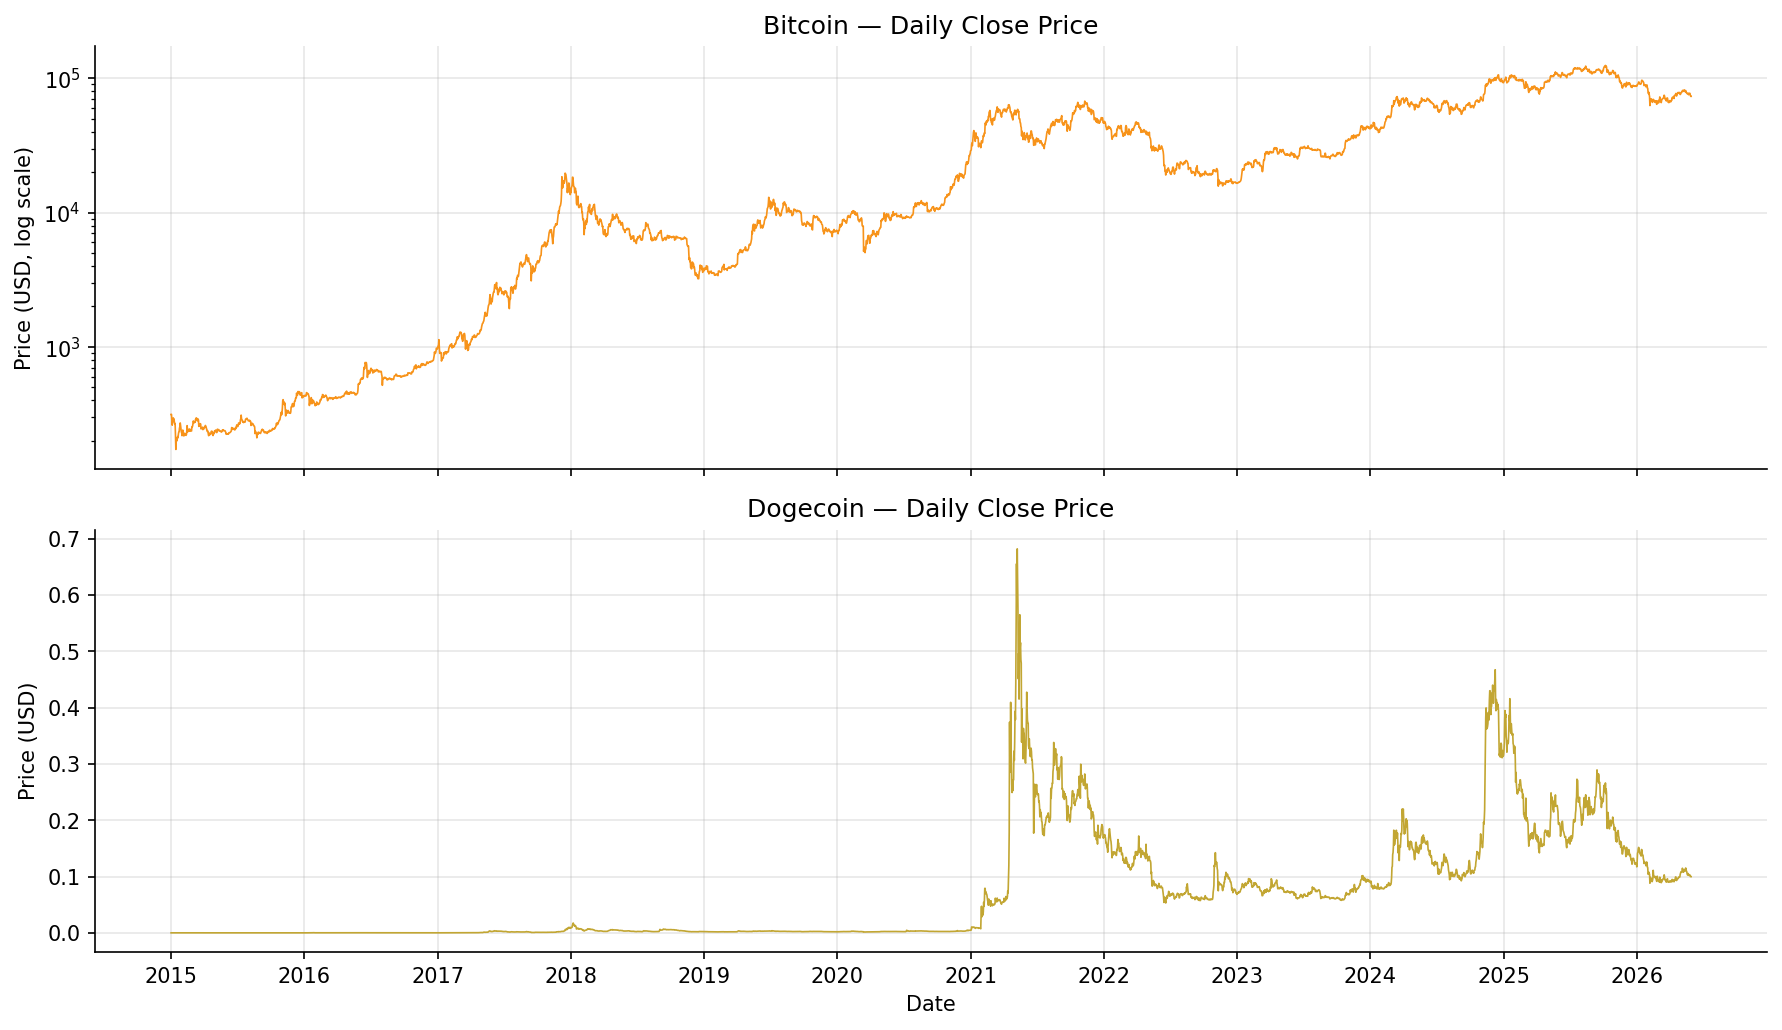
\includegraphics[width=0.95\textwidth]{figures/price_history.png}
  \caption{Lịch sử giá đóng cửa hàng ngày: Bitcoin (log scale, trên) và Dogecoin (tuyến tính, dưới).
           Trục tung BTC dùng log scale do biên độ dao động quá lớn (\$172 đến \$124.753).}
  \label{fig:price_history}
\end{figure}

Hình \ref{fig:price_history} cho thấy một số đặc điểm quan trọng:

\begin{itemize}
  \item \textbf{BTC} tăng trưởng bậc thang với các chu kỳ halving rõ ràng (2017, 2020--2021,
    2024). Biên độ dao động từ mức đỉnh đến đáy (max drawdown) đạt \textbf{--83,64\%}
    trong toàn giai đoạn.
  \item \textbf{DOGE} có đặc tính hoàn toàn khác: phần lớn thời gian dao động dưới \$0,01,
    sau đó có các đợt tăng đột biến theo sự kiện bên ngoài (ví dụ: tweet Elon Musk tháng
    5/2021 đẩy giá lên \$0,68). Max drawdown đạt \textbf{--92,21\%} --- sâu hơn BTC đáng kể.
\end{itemize}

\begin{figure}[H]
  \centering
  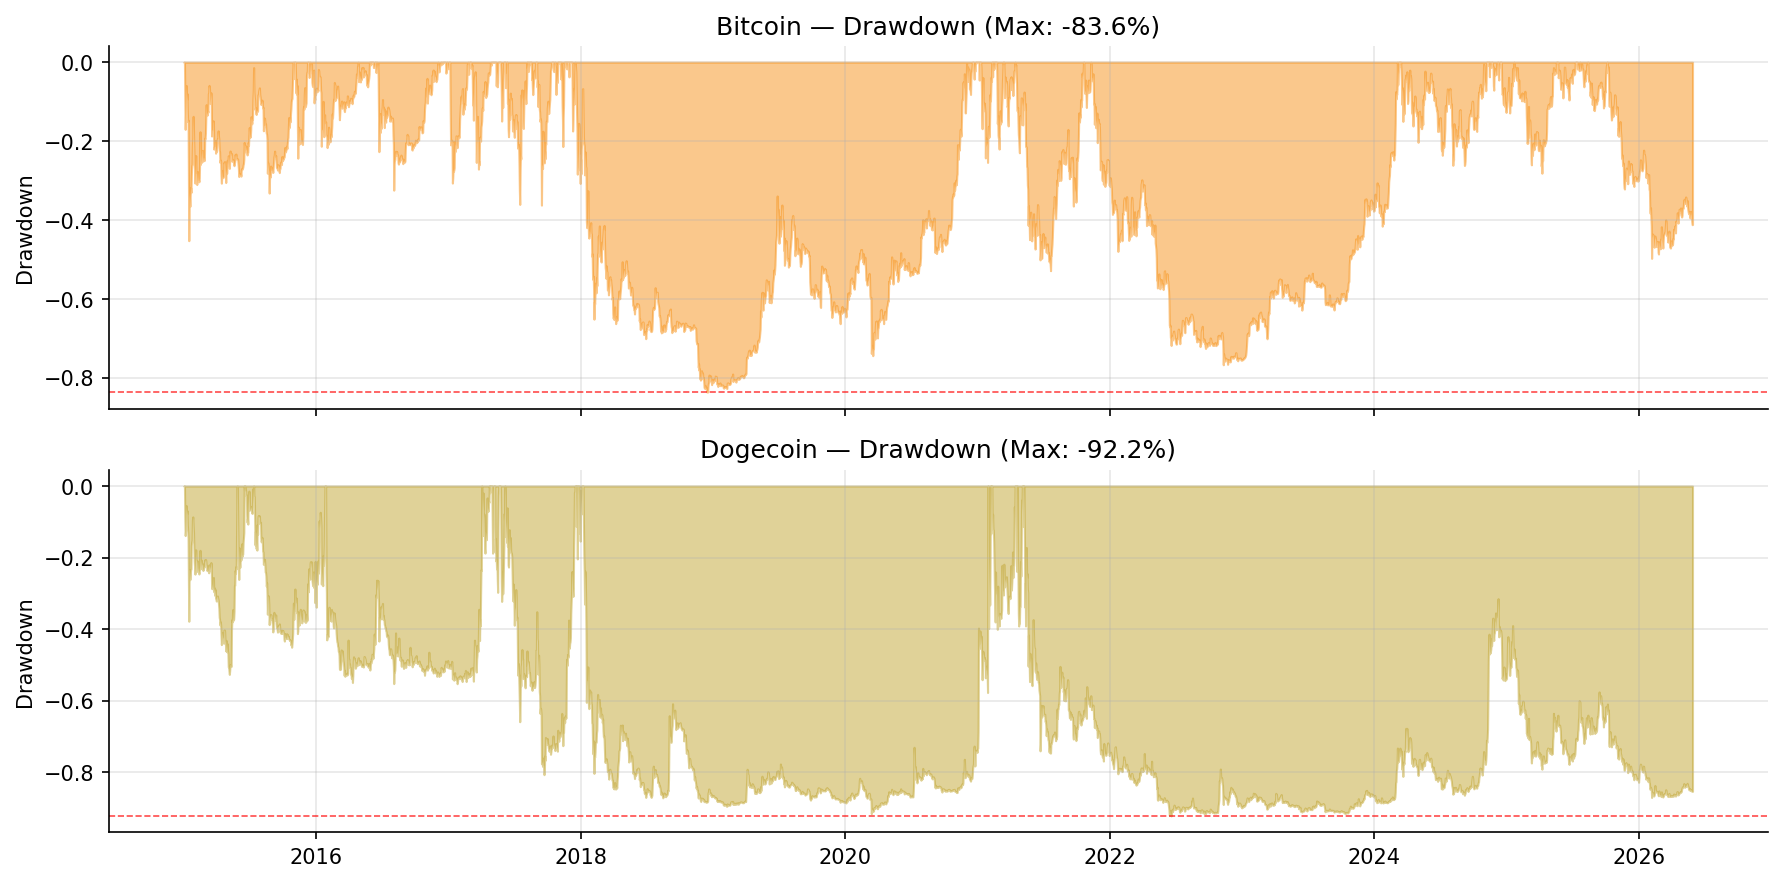
\includegraphics[width=0.95\textwidth]{figures/drawdown_analysis.png}
  \caption{Drawdown analysis: mức sụt giảm so với đỉnh lịch sử. DOGE có các đợt sụt giảm
           sâu hơn và kéo dài hơn BTC, phản ánh tính đầu cơ cao hơn.}
  \label{fig:drawdown}
\end{figure}

\subsection{Phân phối log-return --- lý do không dùng MSE}

\begin{figure}[H]
  \centering
  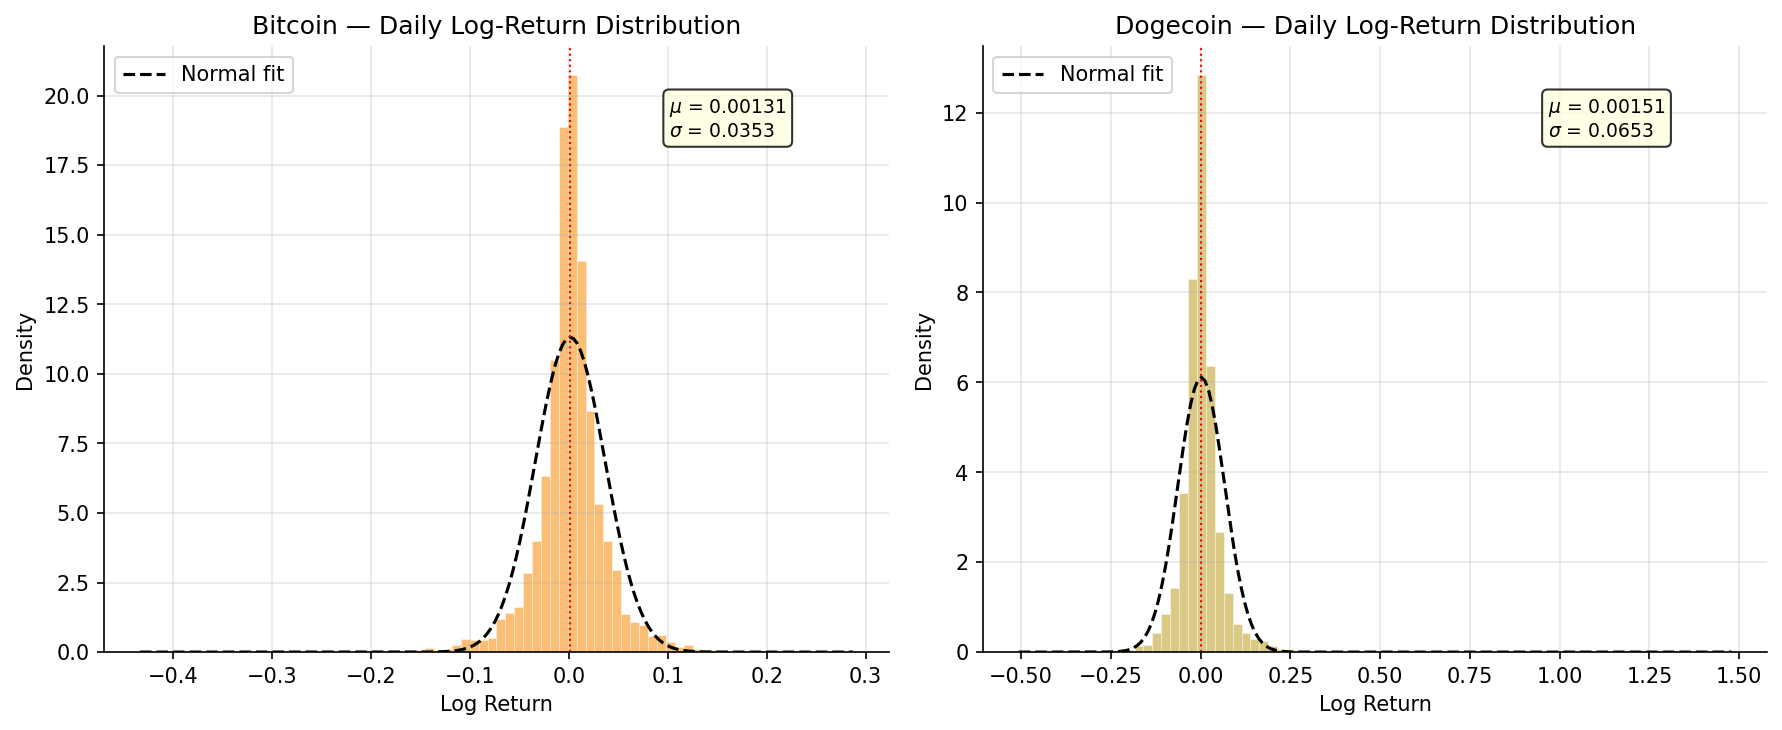
\includegraphics[width=0.95\textwidth]{figures/returns_distribution.png}
  \caption{Phân phối log-return hàng ngày của BTC (trái) và DOGE (phải). Đường nét đứt là
           phân phối chuẩn cùng mean/std. Cả hai đều có \textit{fat tails} rõ ràng.}
  \label{fig:returns_dist}
\end{figure}

Phân tích phân phối log-return trong Hình \ref{fig:returns_dist} và Bảng
\ref{tab:logreturn_stats} là cơ sở quan trọng cho các quyết định thiết kế mô hình:

\begin{table}[H]
  \centering
  \caption{Thống kê log-return hàng ngày}
  \label{tab:logreturn_stats}
  \begin{tabular}{lrrrrr}
    \toprule
    Coin & Mean & Std & Min & Max & Kurtosis \\
    \midrule
    Bitcoin  & +0,001310 & 0,0353 & --0,4337 & +0,2871 & 11,11 \\
    Dogecoin & +0,001514 & 0,0653 & --0,5071 & +1,4791 & 77,02 \\
    \bottomrule
  \end{tabular}
\end{table}

Kurtosis của BTC ($= 11{,}11$) và đặc biệt DOGE ($= 77{,}02$) lớn hơn nhiều so với
phân phối chuẩn ($= 3$), xác nhận hiện tượng \textit{fat tails} (phân phối leptokurtic).
Điều này có nghĩa là các sự kiện cực đoan (crash/pump bất thường) xảy ra thường xuyên
hơn nhiều so với lý thuyết thống kê thông thường dự đoán. Đây là lý do chính để chọn
\textbf{HuberLoss thay vì MSE} trong quá trình huấn luyện: HuberLoss kết hợp $L_2$ cho
sai số nhỏ và $L_1$ cho sai số lớn, giảm thiểu ảnh hưởng của các outlier mà không loại
bỏ chúng hoàn toàn.

\subsection{Kiểm định tính dừng (Stationarity)}

Tính dừng là điều kiện tiên quyết để các đặc trưng thống kê ổn định theo thời gian ---
yêu cầu thiết yếu cho mô hình học sâu. Kiểm định ADF (Augmented Dickey-Fuller) được
áp dụng cho chuỗi giá gốc và chuỗi log-return:

\begin{table}[H]
  \centering
  \caption{Kết quả kiểm định ADF ở mức ý nghĩa $\alpha = 0{,}05$}
  \label{tab:adf}
  \begin{tabular}{llrrr}
    \toprule
    Coin & Chuỗi & ADF Statistic & p-value & Kết luận \\
    \midrule
    Bitcoin  & Giá đóng cửa   & --1,178 & 0,683   & Không dừng \\
    Bitcoin  & Log-return 1 ngày & --66,27 & $\approx 0$ & \textbf{Dừng} \\
    Dogecoin & Giá đóng cửa   & --3,413 & 0,0105  & Dừng (*) \\
    Dogecoin & Log-return 1 ngày & --14,73 & $\approx 0$ & \textbf{Dừng} \\
    \bottomrule
  \end{tabular}
  \begin{flushleft}
  \small (*) DOGE có p-value < 0,05 nhưng đây là kết quả dễ bị ảnh hưởng bởi các đợt pump
  đột biến và không phản ánh tính dừng thực sự của chuỗi giá dài hạn.
  \end{flushleft}
\end{table}

Kết quả khẳng định: chuỗi giá BTC \textbf{không dừng} (random walk), trong khi log-return
của cả hai coin \textbf{dừng mạnh} (p $\approx$ 0). Đây là lý do feature chính của mô hình
là \texttt{log\_return\_1d} thay vì raw close price.

\subsection{Phân tích khối lượng giao dịch}

\begin{figure}[H]
  \centering
  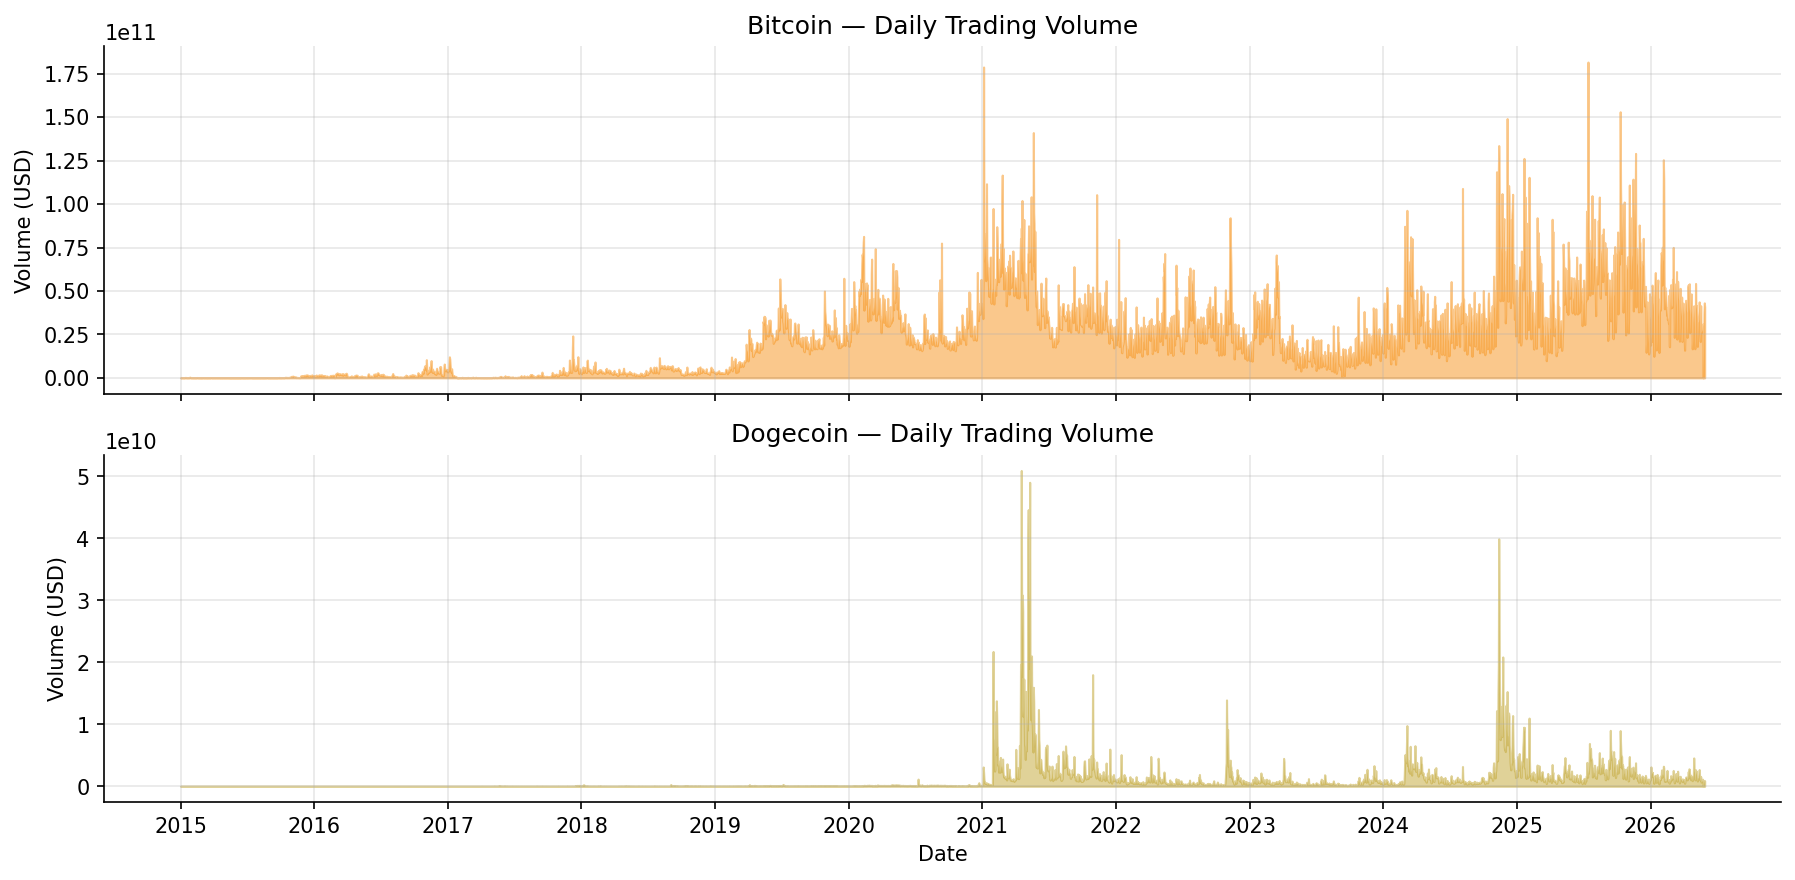
\includegraphics[width=0.95\textwidth]{figures/volume_history.png}
  \caption{Khối lượng giao dịch hàng ngày của BTC (trên) và DOGE (dưới). Đỉnh DOGE năm 2021
           vượt cả BTC trong giai đoạn ngắn, phản ánh cơn sốt đầu cơ.}
  \label{fig:volume}
\end{figure}

Khối lượng giao dịch BTC có xu hướng tăng dài hạn và tương quan với các chu kỳ giá.
DOGE có các đỉnh khối lượng bất thường (tháng 5/2021 đạt \$51 tỷ --- gần bằng đỉnh BTC
cùng giai đoạn) phản ánh bản chất đầu cơ ngắn hạn. Đây là lý do log-return của DOGE
có kurtosis rất cao (77,02).

\subsection{Rolling statistics và xu hướng}

\begin{figure}[H]
  \centering
  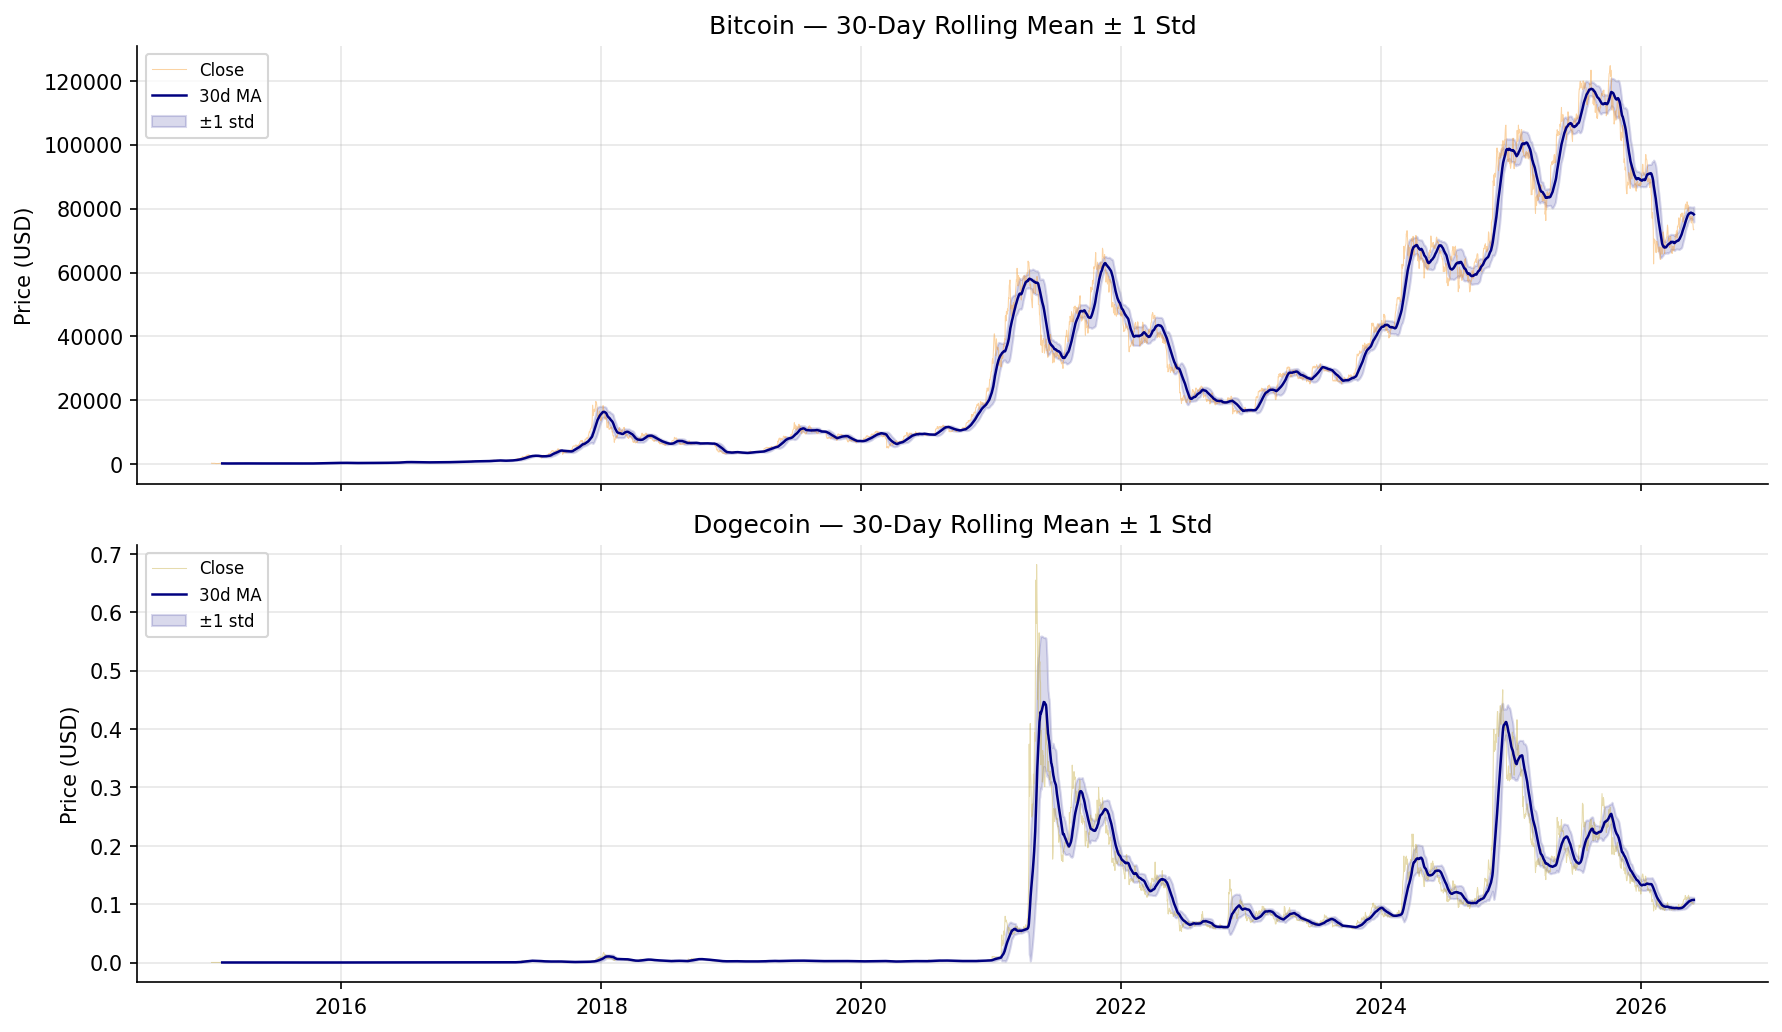
\includegraphics[width=0.95\textwidth]{figures/rolling_statistics.png}
  \caption{Giá đóng cửa (mờ) cùng trung bình trượt 30 ngày $\pm$ 1 độ lệch chuẩn.
           Dải $\pm 1\sigma$ giãn nở mạnh trong các giai đoạn biến động cao.}
  \label{fig:rolling_stats}
\end{figure}

Dải $\pm 1\sigma$ (Hình \ref{fig:rolling_stats}) cho thấy độ biến động của crypto không
đồng nhất theo thời gian (heteroskedastic). Đặc tính này là một phần lý do thêm
\texttt{realized\_vol\_14d} vào bộ features --- để mô hình có thể ``nhìn thấy'' trạng
thái biến động hiện tại và điều chỉnh dự báo tương ứng.

% ------------------------------------------------------------
\section{Tương quan Bitcoin -- Dogecoin}

\begin{figure}[H]
  \centering
  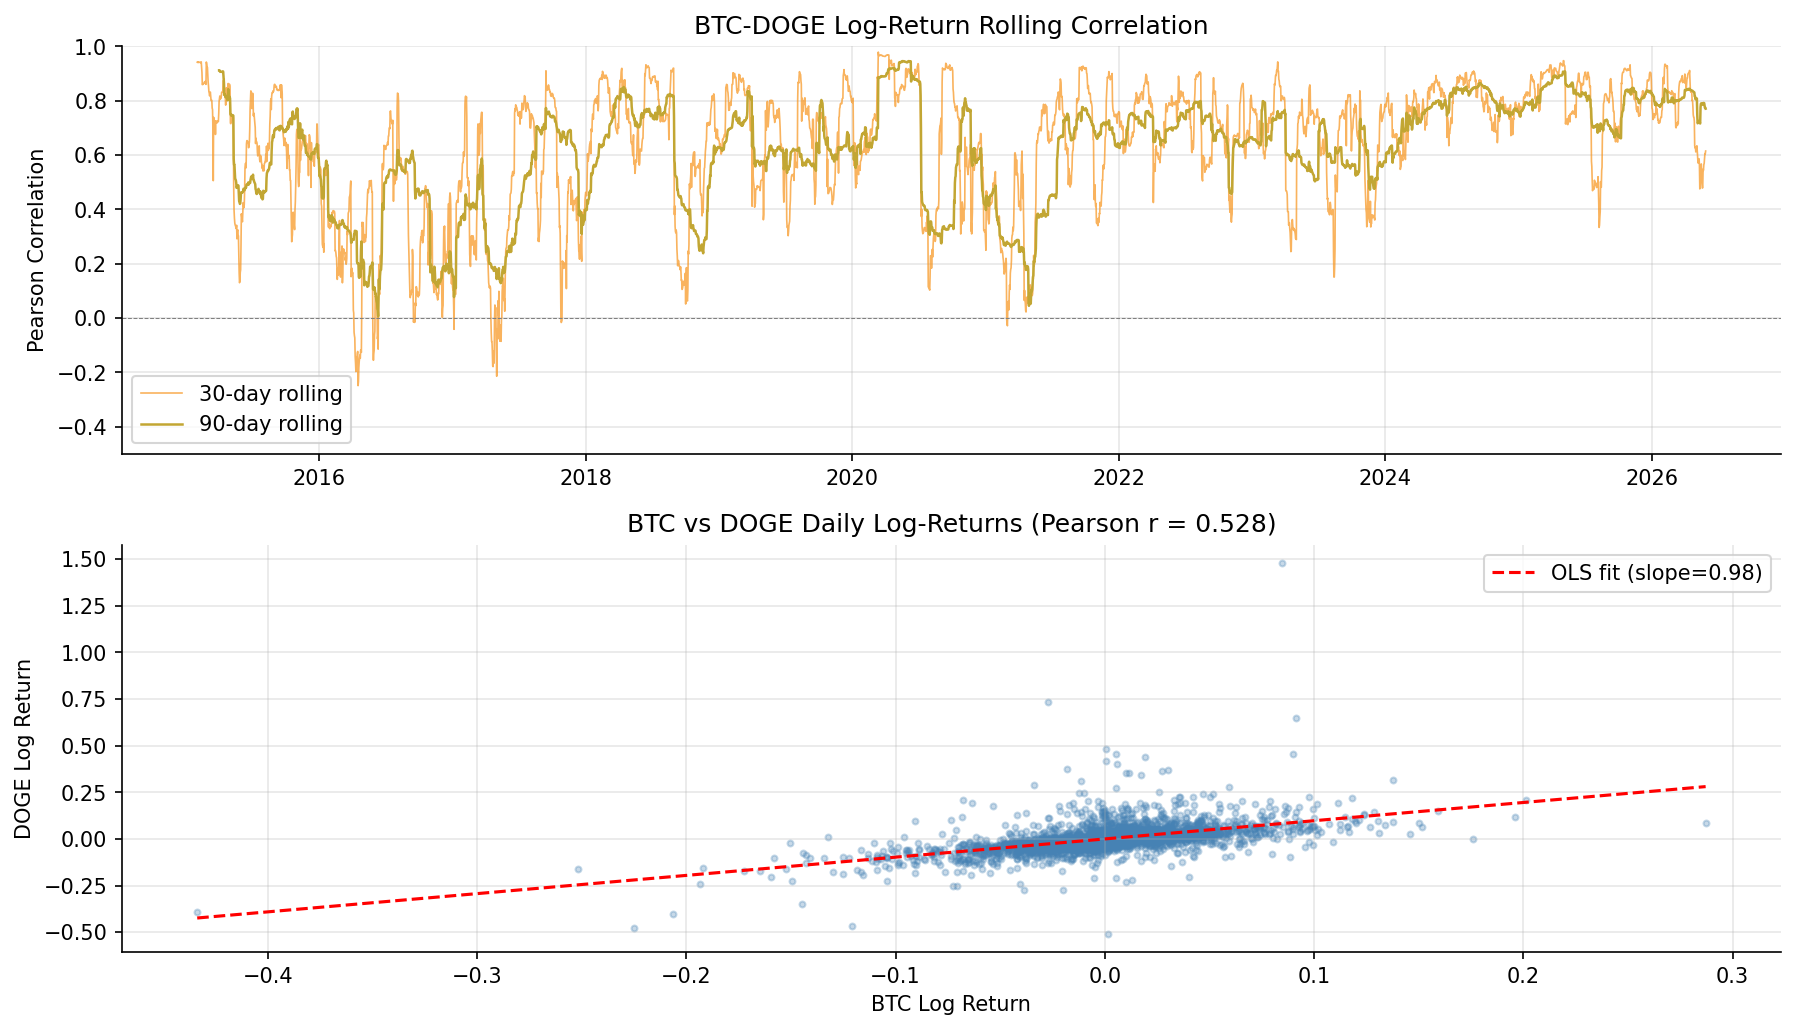
\includegraphics[width=0.95\textwidth]{figures/btc_doge_correlation.png}
  \caption{Trên: tương quan Pearson trượt 30 ngày và 90 ngày giữa log-return BTC và DOGE.
           Dưới: scatter plot log-return hàng ngày với đường hồi quy OLS.}
  \label{fig:correlation}
\end{figure}

Kết quả phân tích tương quan:
\begin{itemize}
  \item \textbf{Tương quan tổng thể:} Pearson $r = 0{,}528$ --- tương quan dương vừa phải,
    không đủ cao để mô hình một coin có thể thay thế cho coin kia.
  \item \textbf{Tương quan trượt 30 ngày (trung bình):} $r = 0{,}637$ --- trong ngắn hạn,
    hai coin thường di chuyển cùng chiều do ảnh hưởng của dòng tiền chung vào thị trường.
  \item \textbf{Biến thiên theo thời gian:} Tương quan dao động mạnh (từ dưới 0,2 đến
    trên 0,8), đặc biệt thấp trong giai đoạn DOGE có pump độc lập (2021). Đây là bằng
    chứng rõ ràng rằng \textbf{nên huấn luyện hai mô hình riêng biệt} thay vì một mô
    hình chung cho cả hai coin.
\end{itemize}

% ------------------------------------------------------------
\section{Xây dựng đặc trưng (Feature Engineering)}

\subsection{Thiết kế bộ đặc trưng 9 chiều}

Một trong những quyết định quan trọng nhất của đề tài là chọn \textbf{9 đặc trưng kỹ thuật}
thay vì dùng raw price. Mục tiêu: tập hợp các tín hiệu bổ sung nhau, đều có tính dừng,
và không có redundancy quá mức.

\begin{table}[H]
  \centering
  \caption{Bộ 9 đặc trưng đầu vào --- định nghĩa, giá trị thực tế (BTC) và lý do chọn}
  \label{tab:features}
  \begin{tabular}{clrrl}
    \toprule
    \# & Tên feature & Mean & Std & Lý do / Vai trò \\
    \midrule
    0 & \texttt{log\_return\_1d}    & +0,0014 & 0,0347 & Tín hiệu chuỗi thời gian chính, dừng \\
    1 & \texttt{momentum\_30d}      & +0,0236 & 0,1163 & Xu hướng trung hạn (SMA30 relative) \\
    2 & \texttt{realized\_vol\_14d} & +0,0305 & 0,0165 & Trạng thái biến động hiện tại \\
    3 & \texttt{RSI\_14}            & 53,38  & 13,81  & Overbought/oversold momentum \\
    4 & \texttt{log\_volume}        & 22,79  & 2,07   & Xác nhận breakout qua khối lượng \\
    5 & \texttt{macd\_norm}         & +0,0047 & 0,0420 & Động lượng ngắn vs. dài hạn \\
    6 & \texttt{bb\_pct\_b}         & 0,555  & 0,337  & Vị trí trong Bollinger Band \\
    7 & \texttt{atr\_norm}          & +0,0227 & 0,0263 & Proxy ATR --- biên độ dao động tức thì \\
    8 & \texttt{fear\_greed}        & 0,5    & 0      & Sentiment (placeholder khi không có data) \\
    \bottomrule
  \end{tabular}
\end{table}

\textbf{Giải thích các quyết định quan trọng:}

\begin{itemize}
  \item \texttt{momentum\_30d} ($= \text{close}/\text{SMA}_{30} - 1$) thay thế
    \texttt{log\_return\_7d} từ v1. Lý do: log-return 7 ngày quá tương quan với
    \texttt{log\_return\_1d} (redundancy), trong khi momentum so với SMA30 nắm bắt xu
    hướng trung hạn độc lập hơn.

  \item \texttt{realized\_vol\_14d} (rolling std của log-return 14 ngày) được thêm ở v3
    thay cho \texttt{log\_return\_30d}. Đây là input trực tiếp cho volatility head --- mô
    hình cần ``biết'' trạng thái biến động gần đây để dự đoán biến động tương lai.

  \item \texttt{atr\_norm} dùng $|\text{log\_return\_1d}|$ thay vì ATR thực sự (cần
    high/low giá). Dữ liệu CoinGecko daily chỉ có close/volume, không có OHLC đầy đủ.
    Đây là \textbf{giới hạn của nguồn dữ liệu} cần cải thiện trong tương lai.

  \item \texttt{fear\_greed} hiện tại = 0,5 (neutral) khi không tải được Fear \& Greed
    Index. Feature này là placeholder, chưa mang thông tin thực sự vào mô hình hiện tại.
\end{itemize}

\subsection{Phân tích đặc trưng trực quan}

\begin{figure}[H]
  \centering
  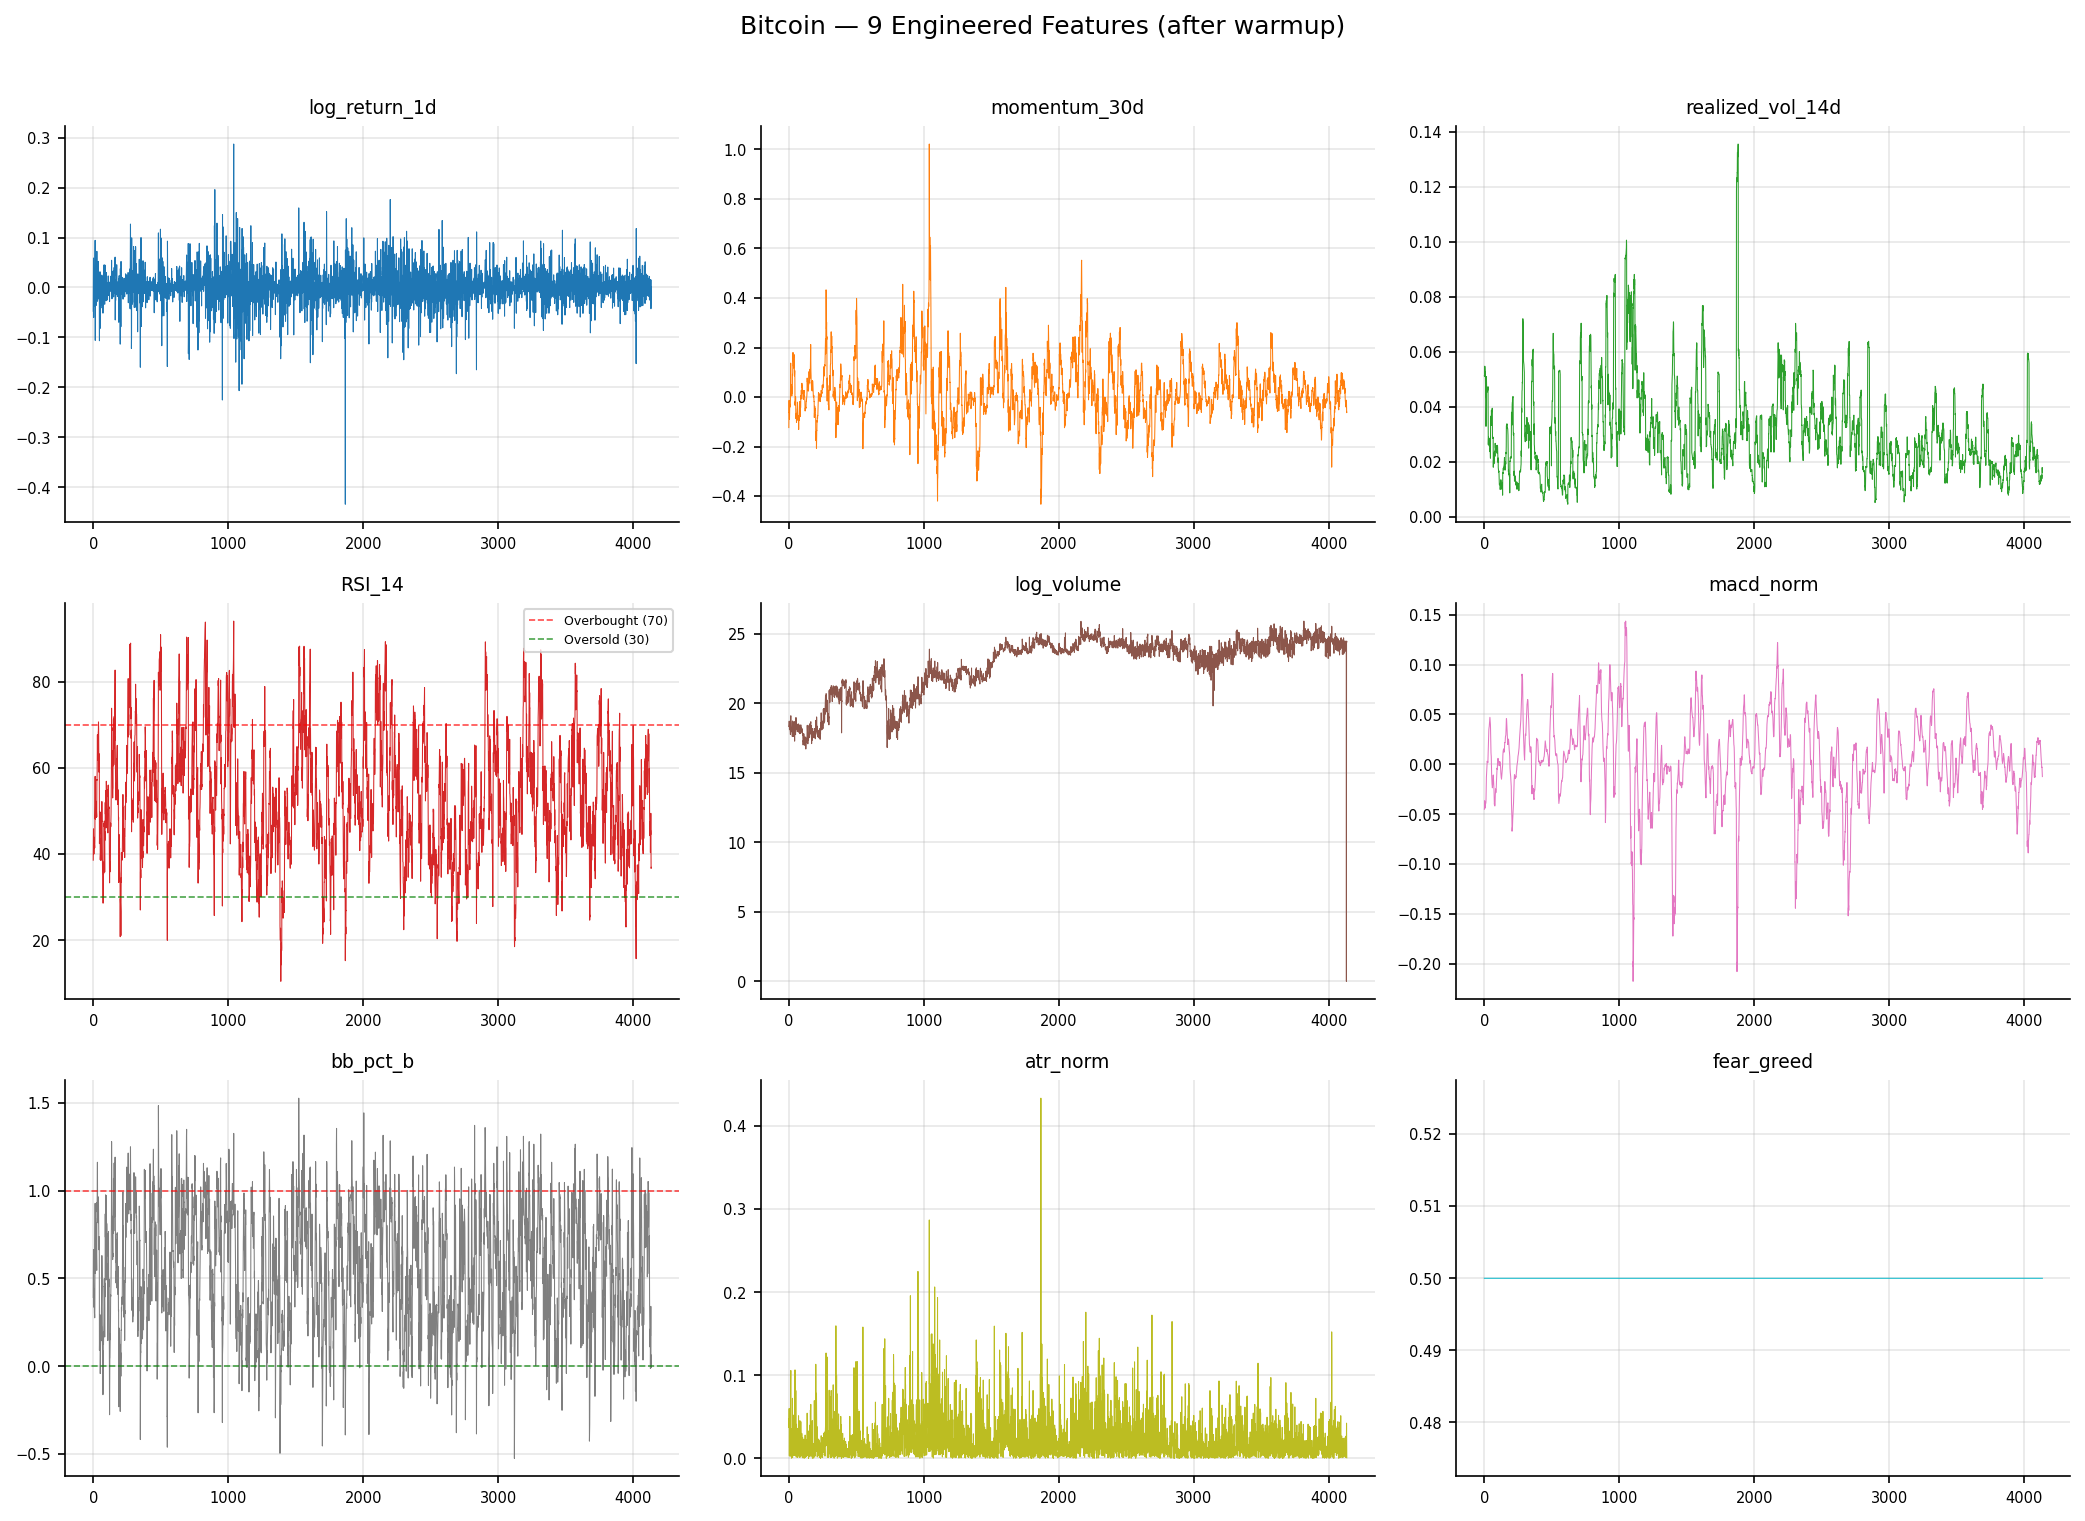
\includegraphics[width=\textwidth]{figures/feature_panel_btc.png}
  \caption{Chuỗi thời gian của 9 đặc trưng cho Bitcoin (sau khi loại bỏ 29 hàng warmup).
           RSI\_14 thêm đường ngưỡng 30 và 70; bb\_pct\_b thêm ranh giới dải Bollinger.}
  \label{fig:feature_panel}
\end{figure}

\begin{figure}[H]
  \centering
  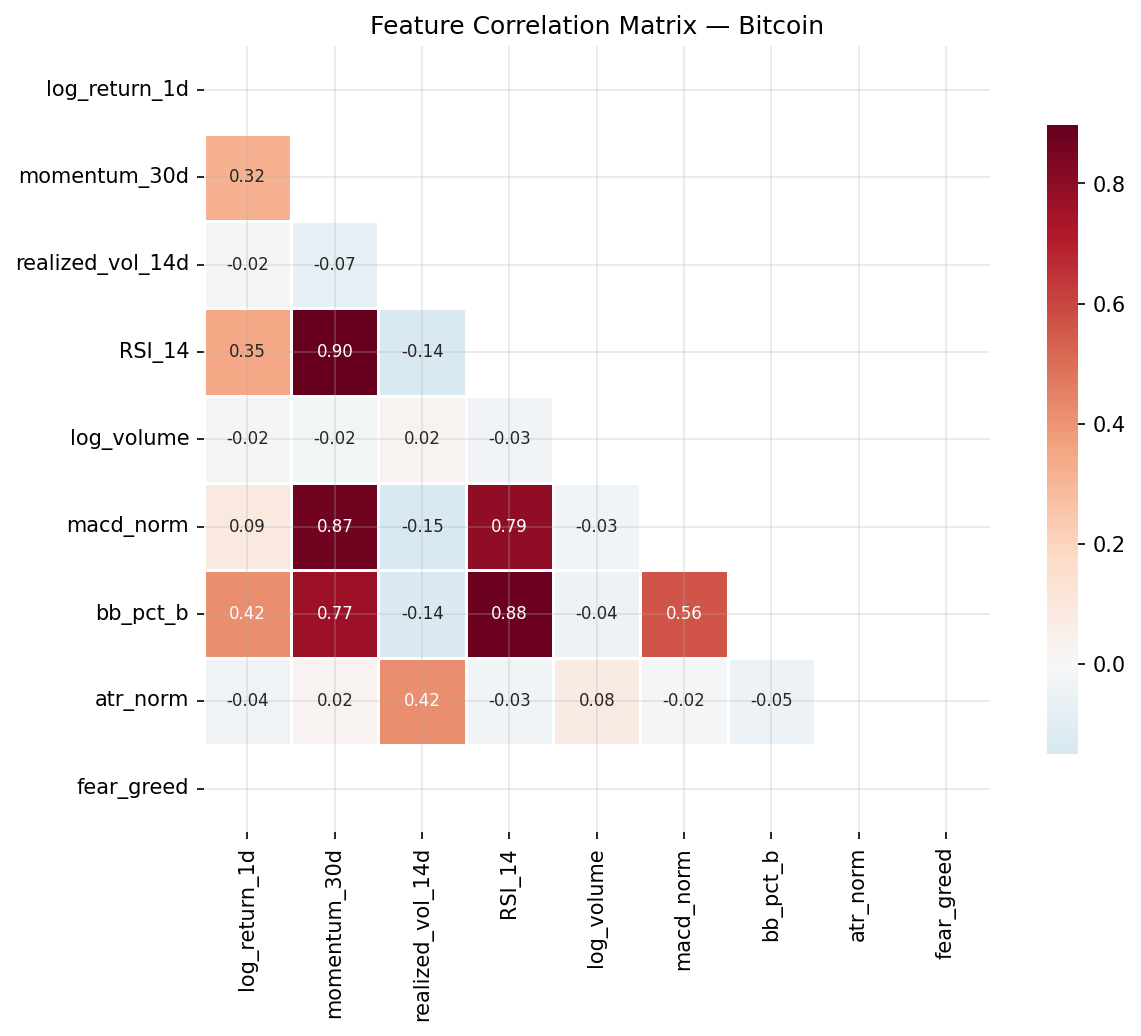
\includegraphics[width=0.85\textwidth]{figures/feature_correlation_heatmap.png}
  \caption{Ma trận tương quan Pearson giữa 9 đặc trưng (Bitcoin). Giá trị dương = màu đỏ,
           âm = màu xanh. Tương quan cao nhất giữa \texttt{atr\_norm} và
           \texttt{realized\_vol\_14d} ($r \approx 0{,}7$) là chấp nhận được vì cả hai
           đo biến động, nhưng ở thang thời gian khác nhau (tức thì vs. 14 ngày).}
  \label{fig:feat_corr}
\end{figure}

Hình \ref{fig:feat_corr} cho thấy phần lớn các feature có tương quan thấp với nhau ---
đây là tính chất mong muốn. Ngoại lệ duy nhất đáng chú ý là \texttt{atr\_norm} và
\texttt{realized\_vol\_14d} có tương quan cao ($r \approx 0{,}7$). Hai feature này đều
đo volatility nhưng ở thang thời gian khác: \texttt{atr\_norm} phản ánh biến động tức
thì của ngày hôm đó, còn \texttt{realized\_vol\_14d} là trung bình 14 ngày. Sự redundancy
vừa phải này được chấp nhận vì volatility head cần cả hai thang thời gian để hoạt động.

\subsection{Warmup và số hàng hợp lệ}

Việc tính SMA30 yêu cầu ít nhất 30 quan sát liên tiếp, đây là constraint lớn nhất trong
bộ feature. Sau khi loại bỏ 29 hàng warmup, bộ dữ liệu còn lại
$4.165 - 29 = \mathbf{4.136}$ hàng hợp lệ.

% ------------------------------------------------------------
\section{Phân chia tập dữ liệu}

\subsection{Nguyên tắc phân chia chronological}

Không giống các bài toán phân loại thông thường, dữ liệu chuỗi thời gian \textbf{tuyệt
đối không được shuffle} trước khi chia train/val/test. Việc shuffle gây ra
\textbf{data leakage}: mô hình có thể ``thấy'' tương lai trong quá trình huấn luyện,
dẫn đến overfitting và kết quả đánh giá sai lệch.

Hệ thống sử dụng \textbf{phân chia tuần tự theo thứ tự thời gian} với tỷ lệ
\textbf{80/10/10}:

\begin{figure}[H]
  \centering
  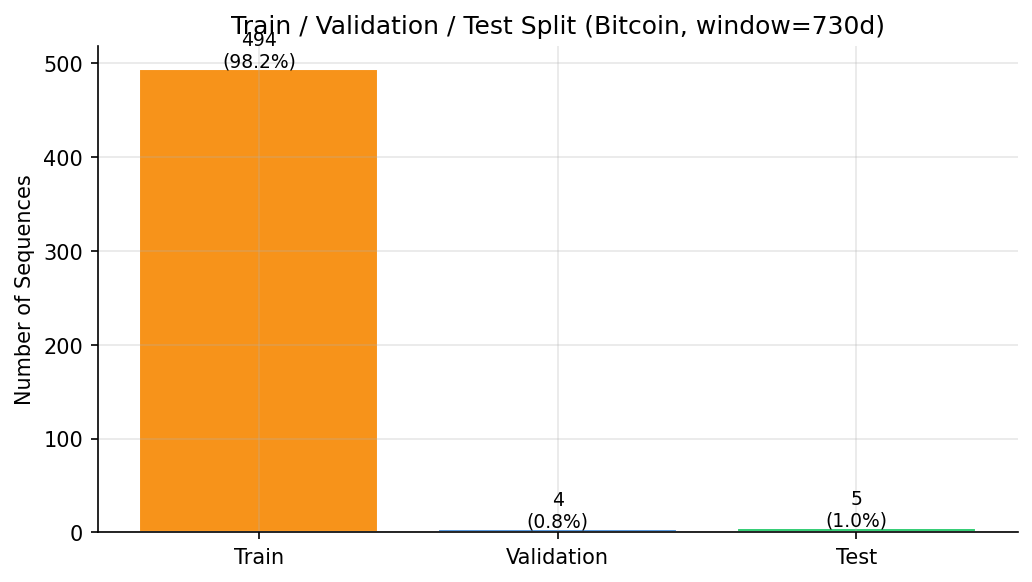
\includegraphics[width=0.75\textwidth]{figures/train_val_test_split.png}
  \caption{Phân bố số lượng chuỗi input trong ba tập dữ liệu (cửa sổ training 730 ngày).
           Tập validation và test mỗi tập tương ứng khoảng 73 ngày liên tiếp cuối cùng
           của cửa sổ.}
  \label{fig:split}
\end{figure}

\subsection{Rolling window và cơ chế phân chia}

Để tránh mô hình bị áp đảo bởi dữ liệu quá cũ (crypto thay đổi regime nhanh), hệ thống
áp dụng tham số \texttt{window\_days}: chỉ sử dụng \textbf{730 ngày gần nhất} (2 năm)
làm cửa sổ huấn luyện. Sau đó, cửa sổ này được chia tuần tự:

\begin{itemize}
  \item \textbf{Train:} 80\% đầu tiên (khoảng 584 ngày)
  \item \textbf{Validation:} 10\% tiếp theo (~73 ngày) --- dùng để early stopping
  \item \textbf{Test:} 10\% cuối (~73 ngày) --- dùng để báo cáo kết quả cuối cùng
\end{itemize}

Mỗi chuỗi input $\mathbf{X}$ có shape $(60, 9)$ --- 60 ngày lịch sử $\times$ 9 feature.
Mỗi target $\mathbf{y}$ là vector 7 log-return tương lai tương ứng (MIMO 7-step forecast).

\subsection{Phân phối nhãn hướng (direction labels)}

\begin{figure}[H]
  \centering
  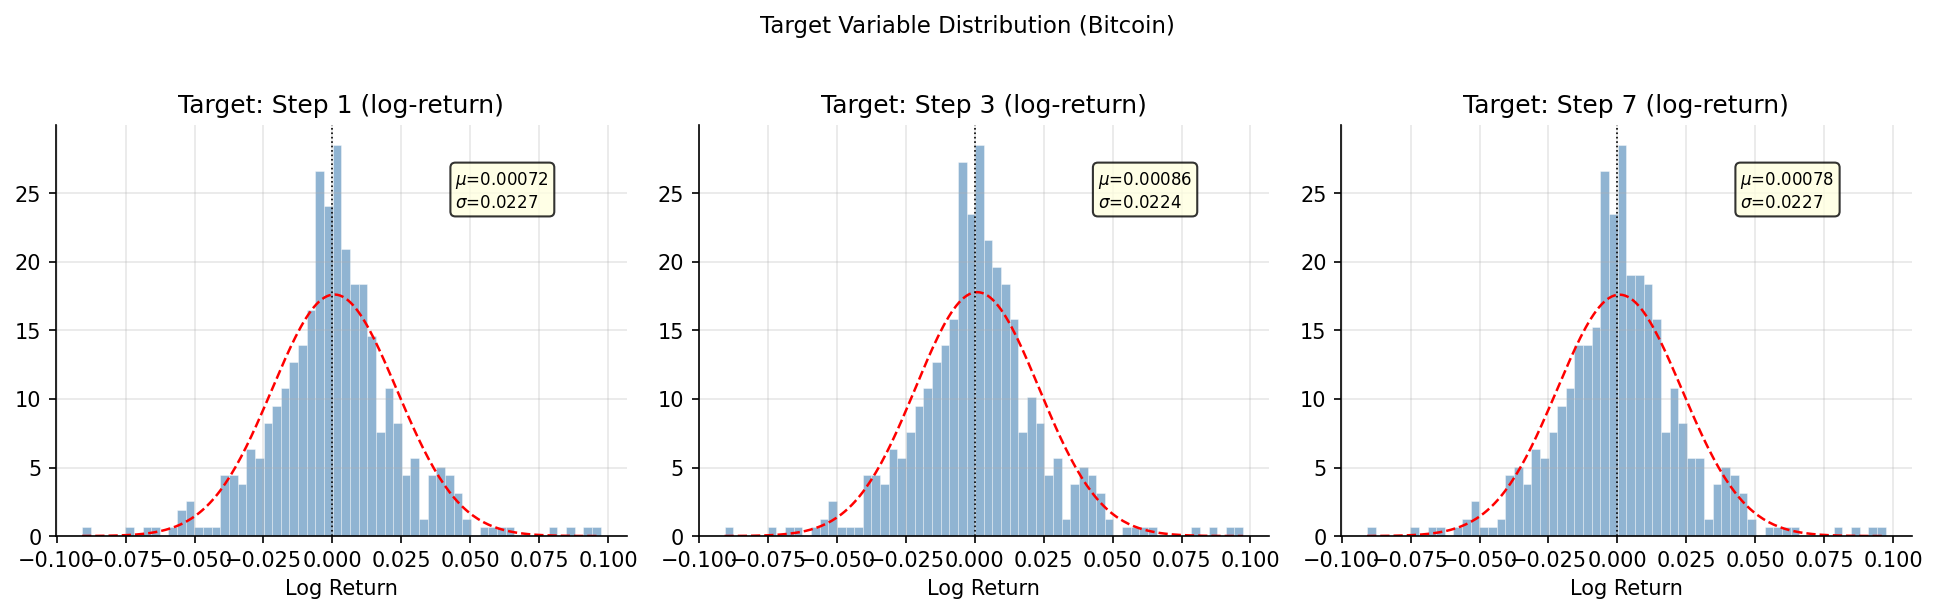
\includegraphics[width=0.9\textwidth]{figures/target_distribution.png}
  \caption{Phân phối target log-return tại bước 1, 3, 7 ngày (Bitcoin). Phương sai tăng
           dần theo horizon, cho thấy bài toán dự đoán bước 7 khó hơn đáng kể.}
  \label{fig:target_dist}
\end{figure}

Nhãn hướng UP/DOWN được tạo bằng \textbf{adaptive-threshold labelling} dựa trên median
của training set:

\begin{center}
$y_{\text{dir}}[k] = \begin{cases} 1 \text{ (UP)} & \text{nếu } y[k] > \text{median}(y_{\text{train}}[:, k]) \\ 0 \text{ (DOWN)} & \text{ngược lại} \end{cases}$
\end{center}

Kết quả là phân phối nhãn \textbf{gần như cân bằng hoàn toàn} (Step 1: UP=50,5\%,
Step 3: UP=51,1\%, Step 7: UP=50,7\%), tránh được class imbalance problem. Tuy nhiên,
đây cũng có nghĩa là ngưỡng UP/DOWN là \textit{tương đối so với median} --- không phải
tăng/giảm tuyệt đối theo giá gốc. Điều này cần lưu ý khi diễn giải kết quả directional
accuracy.

% ------------------------------------------------------------
\section{Tóm tắt chương}

\begin{itemize}
  \item Bộ dữ liệu gồm \textbf{4.165 quan sát/coin} trải dài 11,4 năm (2015--2026), chất
    lượng tốt (dưới 0,03\% null).
  \item Log-return của cả hai coin \textbf{dừng mạnh} (ADF p $\approx$ 0), xác nhận đây
    là không gian feature phù hợp. Raw price không dừng (BTC: p = 0,683).
  \item DOGE có \textbf{fat tails cực đoan} (kurtosis = 77) và \textbf{max drawdown --92\%},
    đặt ra thách thức lớn hơn cho mô hình dự đoán so với BTC.
  \item BTC-DOGE có tương quan vừa phải ($r = 0{,}528$) và biến thiên mạnh theo thời
    gian $\rightarrow$ cần hai mô hình riêng biệt.
  \item Bộ \textbf{9 feature} được thiết kế để bổ sung nhau: momentum, volatility,
    technical indicators, và volume --- mỗi loại nắm bắt một khía cạnh khác nhau của
    động lực giá.
  \item Feature \texttt{fear\_greed} hiện là placeholder 0,5 --- đây là điểm cần cải
    thiện trong các phiên bản tiếp theo.
\end{itemize}

% ============================================================
\chapter{PHƯƠNG PHÁP ĐỀ XUẤT}

\section{Tổng quan kiến trúc Lambda}

Kiến trúc Lambda của hệ thống chia luồng xử lý thành ba lớp rõ ràng, mỗi lớp phục
vụ một mục tiêu khác biệt về độ trễ và độ chính xác:

\begin{itemize}
  \item \textbf{Batch Layer:} Apache Spark Batch xử lý toàn bộ dữ liệu lịch sử từ CSV,
    tính toán các bộ tập hợp có độ trễ cao nhưng chính xác: \texttt{daily\_stats}
    (OHLCV hàng ngày), \texttt{historical\_sma} (SMA qua nhiều cửa sổ), và
    \texttt{coin\_correlation} (tương quan BTC-DOGE theo thời gian).
  \item \textbf{Speed Layer:} Kafka Producer thu thập dữ liệu giá theo thời gian thực từ
    CoinGecko (mỗi 10 phút), Spark Structured Streaming tiêu thụ topic \texttt{crypto\_raw},
    tính các chỉ số kỹ thuật trên cửa sổ 5 phút và ghi vào MongoDB collection
    \texttt{realtime\_prices}.
  \item \textbf{Serving Layer:} MongoDB lưu trữ kết quả từ cả hai lớp trên. FastAPI (port
    8000) cung cấp REST API với JWT authentication, phục vụ React frontend (port 3000)
    và Streamlit dashboard (port 8501). LSTM Inference Scheduler chạy định kỳ mỗi 5 phút,
    ghi dự đoán 7 ngày vào collection \texttt{predictions}.
\end{itemize}

Luồng dữ liệu hoàn chỉnh được tóm tắt như sau:

\begin{center}
\texttt{CoinGecko API} $\rightarrow$ \texttt{Kafka (crypto\_raw)} $\rightarrow$
\texttt{Spark Streaming} $\rightarrow$ \texttt{MongoDB} $\rightarrow$
\texttt{FastAPI} $\rightarrow$ \texttt{React / Streamlit}
\end{center}

\begin{center}
\texttt{CSV lịch sử} $\rightarrow$ \texttt{Spark Batch} $\rightarrow$
\texttt{MongoDB} $\rightarrow$ \texttt{FastAPI}
\end{center}

\begin{center}
\texttt{CSV lịch sử} $\rightarrow$ \texttt{LSTM Training} $\rightarrow$
\texttt{Inference Scheduler} $\rightarrow$ \texttt{MongoDB (predictions)}
\end{center}

% ------------------------------------------------------------
\section{Speed Layer: Kafka và Spark Streaming}

\subsection{Kafka Producer}

Producer được cấu hình với các tham số đảm bảo độ tin cậy cao:
\texttt{acks=all}, \texttt{retries=3}, \texttt{linger\_ms=100}. Mỗi message
là JSON chứa giá hiện tại, khối lượng, market cap và timestamp UTC.

\subsection{Spark Structured Streaming}

Spark đọc từ Kafka với Structured Streaming API, xử lý dữ liệu qua cửa sổ trượt
5 phút với watermark 10 phút cho dữ liệu trễ. Kết quả được ghi vào MongoDB thông qua
\texttt{foreachBatch} pattern (không dùng streaming sink trực tiếp để đảm bảo
idempotency). Các chỉ số kỹ thuật được tính trong Spark:

\begin{table}[H]
  \centering
  \caption{Các chỉ số kỹ thuật tính toán trong Spark Streaming}
  \label{tab:indicators}
  \begin{tabular}{llp{7cm}}
    \toprule
    Chỉ số & Công thức & Ý nghĩa \\
    \midrule
    SMA-$n$ & $\displaystyle\frac{1}{n}\sum_{i=0}^{n-1} p_{t-i}$ & Trung bình động $n$ kỳ \\[8pt]
    RSI-14  & $100 - \dfrac{100}{1 + \overline{U_{14}}/\overline{D_{14}}}$ & Sức mạnh tương đối (overbought $>$70, oversold $<$30) \\[8pt]
    BB      & $\text{SMA}_{20} \pm 2\sigma_{20}$ & Dải Bollinger --- phát hiện breakout \\[4pt]
    VWAP    & $\displaystyle\frac{\sum p_i v_i}{\sum v_i}$ & Giá trung bình theo khối lượng \\[8pt]
    ATR-14  & $\displaystyle\frac{1}{14}\sum_{i=1}^{14} \text{TR}_i$ & Biên độ dao động thực (True Range) \\
    \bottomrule
  \end{tabular}
\end{table}

% ------------------------------------------------------------
\section{Batch Layer: Spark Batch Job}

Spark Batch Job xử lý toàn bộ dữ liệu CSV (hàng triệu dòng nếu mở rộng) với DataFrame
API, tính và ghi ba collection vào MongoDB:

\begin{itemize}
  \item \texttt{daily\_stats}: Tổng hợp OHLCV hàng ngày với các thống kê mô tả.
  \item \texttt{historical\_sma}: SMA theo nhiều cửa sổ (7, 30, 90, 200 ngày).
  \item \texttt{coin\_correlation}: Rolling Pearson correlation giữa BTC và DOGE
    theo cửa sổ 30 và 90 ngày.
\end{itemize}

% ------------------------------------------------------------
\section{Mô hình LSTM Dual-Head (v3)}

\subsection{Kiến trúc tổng thể}

Mô hình được xây dựng bằng PyTorch \cite{ref8} với kiến trúc LSTM 2 lớp (stacked LSTM)
và hai đầu ra phụ (auxiliary heads). Thiết kế MIMO (Multiple Input Multiple Output) dự
đoán đồng thời tất cả 7 bước thay vì dự đoán tuần tự từng bước, tránh tích lũy sai số.

\begin{table}[H]
  \centering
  \caption{Thông số kiến trúc mô hình LSTM v3}
  \label{tab:model_arch}
  \begin{tabular}{llr}
    \toprule
    Thành phần & Chi tiết & Tham số \\
    \midrule
    LSTM Layer 1 & input=9, hidden=128, dropout=0,2 & 70.656 \\
    LSTM Layer 2 & input=128, hidden=128, dropout=0,2 & 131.584 \\
    Price Head & Linear(128→64)→ReLU→Dropout(0,1)→Linear(64→7) & 8.711 \\
    Volatility Head & Linear(128→64)→ReLU→Dropout(0,1)→Linear(64→7)→Softplus & 8.711 \\
    \midrule
    \textbf{Tổng} & & \textbf{219.662} \\
    \bottomrule
  \end{tabular}
\end{table}

\begin{figure}[H]
  \centering
  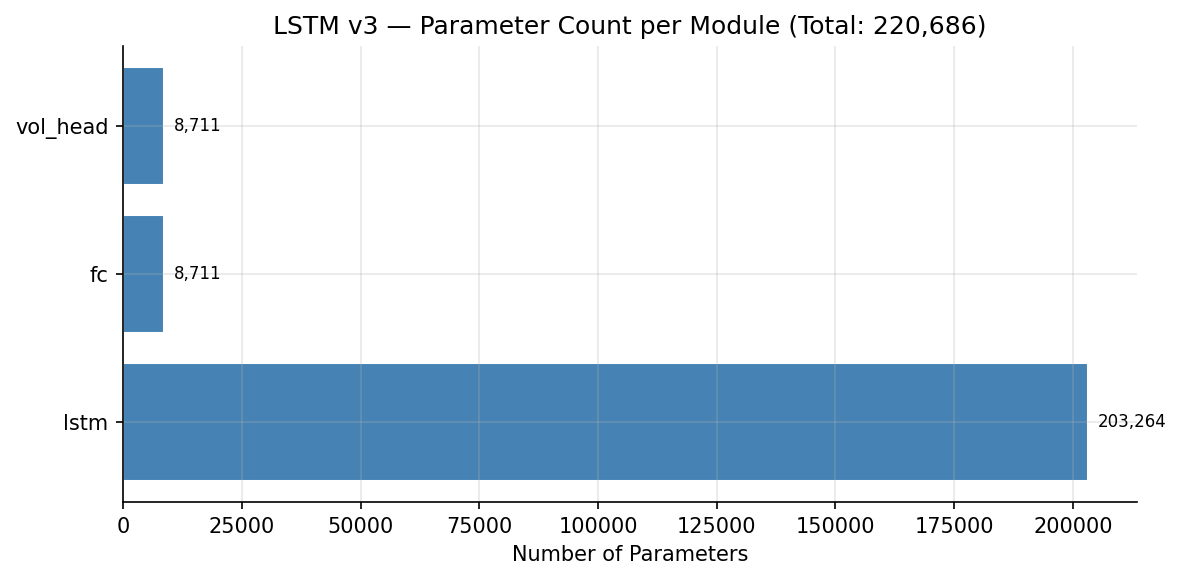
\includegraphics[width=0.7\textwidth]{figures/model_param_counts.png}
  \caption{So sánh số lượng tham số giữa các thành phần của mô hình. LSTM encoder chiếm
           hơn 90\% tổng tham số; các auxiliary heads nhẹ để tránh overfitting.}
  \label{fig:model_params}
\end{figure}

\subsection{LSTM Encoder}

Công thức cập nhật LSTM tại mỗi timestep $t$ \cite{ref4}:

\begin{align}
  f_t &= \sigma(W_f \cdot [h_{t-1}, x_t] + b_f) \quad \text{(forget gate)} \\
  i_t &= \sigma(W_i \cdot [h_{t-1}, x_t] + b_i) \quad \text{(input gate)} \\
  \tilde{C}_t &= \tanh(W_C \cdot [h_{t-1}, x_t] + b_C) \quad \text{(candidate cell)} \\
  C_t &= f_t \odot C_{t-1} + i_t \odot \tilde{C}_t \quad \text{(cell state)} \\
  o_t &= \sigma(W_o \cdot [h_{t-1}, x_t] + b_o) \quad \text{(output gate)} \\
  h_t &= o_t \odot \tanh(C_t) \quad \text{(hidden state)}
\end{align}

Hệ thống sử dụng hidden state cuối cùng $h_{T}$ (với $T = 60$) làm đại diện
cho toàn bộ chuỗi lịch sử 60 ngày, sau đó đưa vào các heads.

\subsection{Price Head và Volatility Head}

\textbf{Price Head} dự đoán vector log-return 7 bước:
$\hat{\mathbf{y}}_{\text{price}} = W_2 \cdot \text{ReLU}(W_1 h_T + b_1) + b_2$,
với shape $(B, 7)$.

\textbf{Volatility Head} dự đoán forward realized volatility 7 bước, đảm bảo
giá trị dương bằng hàm Softplus:
$\hat{\mathbf{y}}_{\text{vol}} = \text{Softplus}(W_4 \cdot \text{ReLU}(W_3 h_T + b_3) + b_4)$,
với shape $(B, 7)$ và $\text{Softplus}(x) = \ln(1 + e^x)$.

\subsection{Hàm mất mát (Loss Function)}

Hàm mất mát kết hợp hai mục tiêu:

\begin{equation}
  \mathcal{L} = \alpha \cdot \mathcal{L}_{\text{price}} + \gamma \cdot \mathcal{L}_{\text{vol}}
\end{equation}

với $\alpha = 1{,}0$, $\gamma = 0{,}3$ (được chọn qua thực nghiệm).

\textbf{Direction-weighted Huber Loss} cho price head:

\begin{equation}
  \mathcal{L}_{\text{price}} = \frac{1}{B \cdot 7} \sum_{b,k}
  w_{b,k} \cdot \ell_\delta(\hat{y}_{b,k} - y_{b,k})
\end{equation}

trong đó $w_{b,k} = 1 + 2 \cdot \mathbb{1}[\text{sign}(\hat{y}) \neq \text{sign}(y)]$
(phạt gấp 3 lần khi dự đoán sai hướng) và $\ell_\delta$ là Huber loss với $\delta = 1$:

\begin{equation}
  \ell_\delta(r) = \begin{cases}
    \frac{1}{2}r^2 & \text{nếu } |r| \leq \delta \\
    \delta(|r| - \frac{1}{2}\delta) & \text{ngược lại}
  \end{cases}
\end{equation}

\textbf{MSE Loss} cho volatility head: $\mathcal{L}_{\text{vol}} = \|\hat{\mathbf{y}}_{\text{vol}} - \mathbf{y}_{\text{vol}}\|_2^2$.

\subsection{Quy trình huấn luyện}

\begin{table}[H]
  \centering
  \caption{Siêu tham số huấn luyện}
  \label{tab:hyperparams}
  \begin{tabular}{lr}
    \toprule
    Siêu tham số & Giá trị \\
    \midrule
    Optimizer & Adam \\
    Learning rate & $10^{-3}$ \\
    Weight decay & $10^{-5}$ \\
    Batch size & 64 \\
    Max epochs & 50 \\
    Early stopping patience & 7 \\
    LR scheduler & ReduceLROnPlateau (factor=0,5, patience=5) \\
    Gradient clipping & max\_norm = 1,0 \\
    \bottomrule
  \end{tabular}
\end{table}

Quá trình huấn luyện sử dụng \textbf{early stopping}: dừng sớm nếu validation loss
không giảm trong 7 epoch liên tiếp. Mô hình tốt nhất (theo val loss) được lưu lại
để dùng cho inference. Gradient clipping với max\_norm = 1,0 ngăn chặn exploding
gradients --- vấn đề phổ biến với LSTM trên dữ liệu tài chính biến động mạnh.

% ------------------------------------------------------------
\section{Walk-Forward Validation}

Walk-forward validation \cite{ref9} là phương pháp đánh giá chuỗi thời gian phù hợp hơn
cross-validation thông thường, vì nó mô phỏng quy trình thực tế: chỉ dùng dữ liệu quá
khứ để dự đoán tương lai.

Hệ thống sử dụng \textbf{6 fold}, mỗi fold gồm 60 ngày validation. Trong mỗi fold:
(1) Huấn luyện một mô hình throwaway trên dữ liệu trước fold đó (trong rolling window
730 ngày); (2) Đánh giá trên 60 ngày validation; (3) Tổng hợp RMSE, MAE và directional
accuracy. Kết quả cuối là trung bình qua 6 fold.

% ============================================================
\chapter{THỰC NGHIỆM VÀ KẾT QUẢ}

\section{Môi trường thực nghiệm}

Hệ thống được triển khai bằng Docker Compose với 9 services trên máy cục bộ:

\begin{table}[H]
  \centering
  \caption{Các services trong Docker Compose}
  \label{tab:services}
  \begin{tabular}{lll}
    \toprule
    Service & Công nghệ & Port \\
    \midrule
    Zookeeper & Apache Zookeeper 3.7 & 2181 \\
    Kafka Broker & Apache Kafka 3.4 & 9092 \\
    Kafka UI & Provectus Kafka UI & 8080 \\
    MongoDB & MongoDB 6.0 & 27017 \\
    Spark Master & Apache Spark 3.5 & 8081 \\
    Spark Worker & Apache Spark 3.5 & -- \\
    Producer & Python (pycoingecko) & -- \\
    Dashboard & Streamlit 1.32 & 8501 \\
    API Backend & FastAPI + Uvicorn & 8000 \\
    Frontend & React 19 + Nginx & 3000 \\
    Inference Scheduler & PyTorch 2.2 & -- \\
    \bottomrule
  \end{tabular}
\end{table}

\textbf{Cấu hình phần cứng thực nghiệm:} CPU Intel Core i7 (8 cores), RAM 16 GB,
lưu trữ SSD. Mô hình LSTM huấn luyện trên CPU (không cần GPU do dataset nhỏ ~3.000 mẫu).

\section{Quy trình thực nghiệm}

\begin{enumerate}
  \item Khởi động infrastructure: \texttt{make docker-up}
  \item Tạo Kafka topics: \texttt{bash scripts/create\_topics.sh}
  \item Điền dữ liệu lịch sử vào MongoDB: \texttt{bash scripts/run\_batch.sh}
  \item Huấn luyện LSTM và chạy inference: \texttt{make infer-all}
  \item Đánh giá backtest 6 tháng: \texttt{python src/ml/backtest\_compare.py}
  \item Xem kết quả qua React frontend (port 3000)
\end{enumerate}

\section{Độ đo đánh giá}

\begin{itemize}
  \item \textbf{RMSE} (Root Mean Squared Error): $\sqrt{\frac{1}{M \cdot 7}\sum_{m,k}(\hat{p}_{m,k} - p_{m,k})^2}$ tính trên giá USD tái tạo.
  \item \textbf{MAE} (Mean Absolute Error): $\frac{1}{M \cdot 7}\sum_{m,k}|\hat{p}_{m,k} - p_{m,k}|$ tính trên giá USD tái tạo.
  \item \textbf{Directional Accuracy}: $\frac{1}{M}\sum_m \mathbb{1}[\text{sign}(\hat{r}_{m,1}) = \text{sign}(r_{m,1})]$ --- đúng hướng bước 1.
  \item \textbf{Walk-Forward Dir Acc}: Trung bình directional accuracy qua 6 fold walk-forward.
\end{itemize}

Lưu ý: RMSE và MAE được tính trên giá USD tái tạo từ cumulative log-return, không phải
trực tiếp trên log-return chuẩn hóa.

\section{Kết quả trên tập kiểm thử}

\subsection{So sánh BTC và DOGE}

\begin{table}[H]
  \centering
  \caption{Kết quả trên tập test (10\% cuối của rolling window 730 ngày, ~73 ngày)}
  \label{tab:test_results}
  \begin{tabular}{lrrrr}
    \toprule
    Coin & RMSE & MAE & Dir Acc (bước 1) & Epochs trained \\
    \midrule
    Bitcoin (BTC) & \$1.799,50 & \$1.288,92 & 40,0\% & 10 \\
    Dogecoin (DOGE) & \$0,00325 & \$0,00267 & 20,0\% & 18 \\
    \bottomrule
  \end{tabular}
\end{table}

\begin{figure}[H]
  \centering
  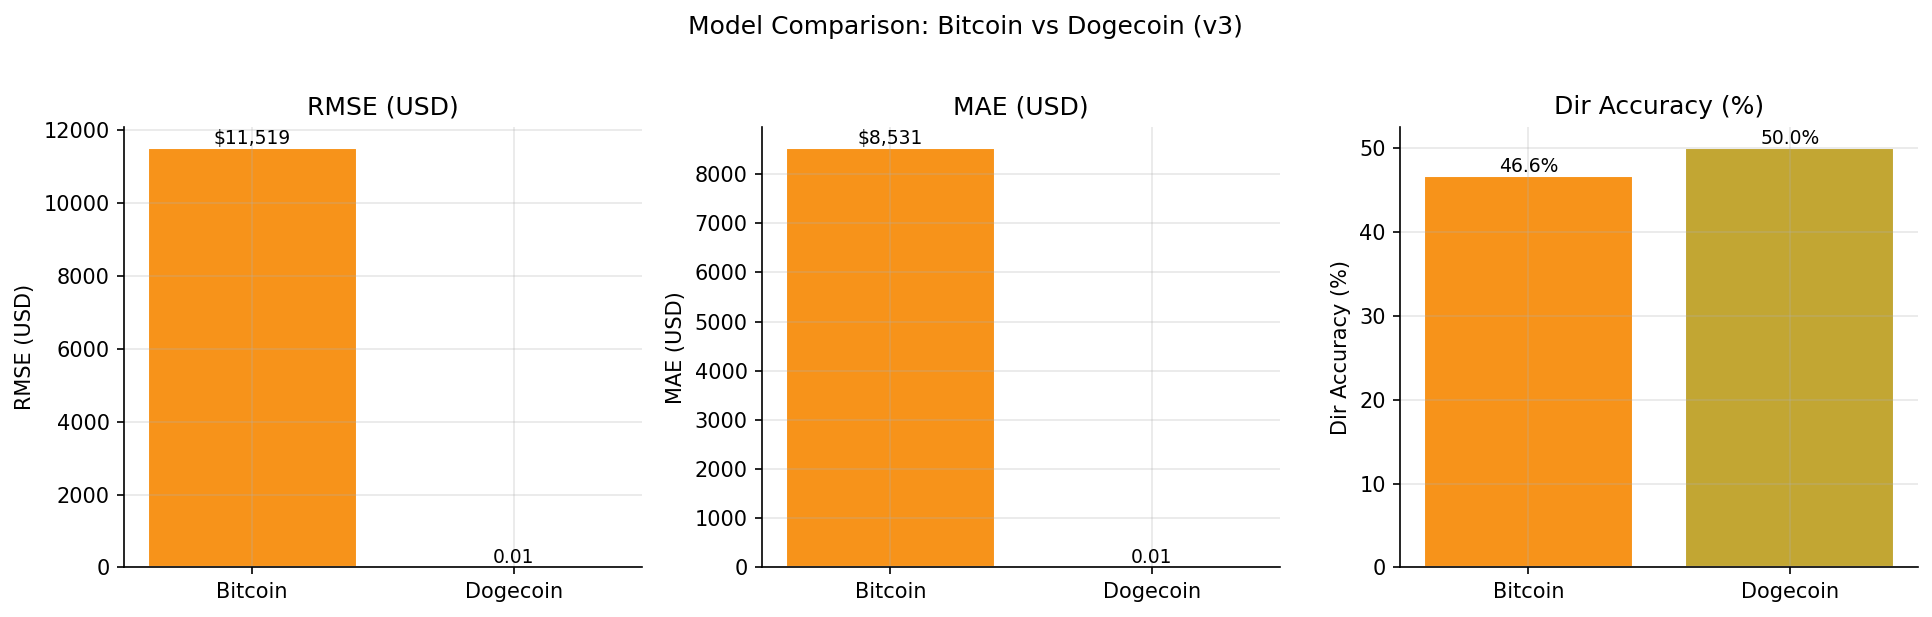
\includegraphics[width=0.95\textwidth]{figures/model_comparison_btc_vs_doge.png}
  \caption{So sánh hiệu suất mô hình BTC và DOGE theo các độ đo. BTC có RMSE tuyệt đối
           lớn hơn nhiều (theo USD) nhưng MAPE thấp hơn DOGE do giá BTC cao hơn.}
  \label{fig:model_compare}
\end{figure}

\textbf{Phân tích:} Directional accuracy thấp (40\% cho BTC, 20\% cho DOGE) trên tập test
thuần túy phản ánh đặc thù của bài toán: mô hình được huấn luyện để tối thiểu hóa
Huber loss trên log-return, không trực tiếp tối đa hóa directional accuracy. Hơn nữa,
tập test chỉ có $\sim$73 quan sát --- đủ nhỏ để kết quả có thể dao động lớn theo thời
kỳ thị trường. Kết quả walk-forward (nhiều fold, dữ liệu đa dạng hơn) đáng tin cậy hơn
để đánh giá tổng quát.

\subsection{Phân tích MAE theo từng bước dự đoán}

\begin{figure}[H]
  \centering
  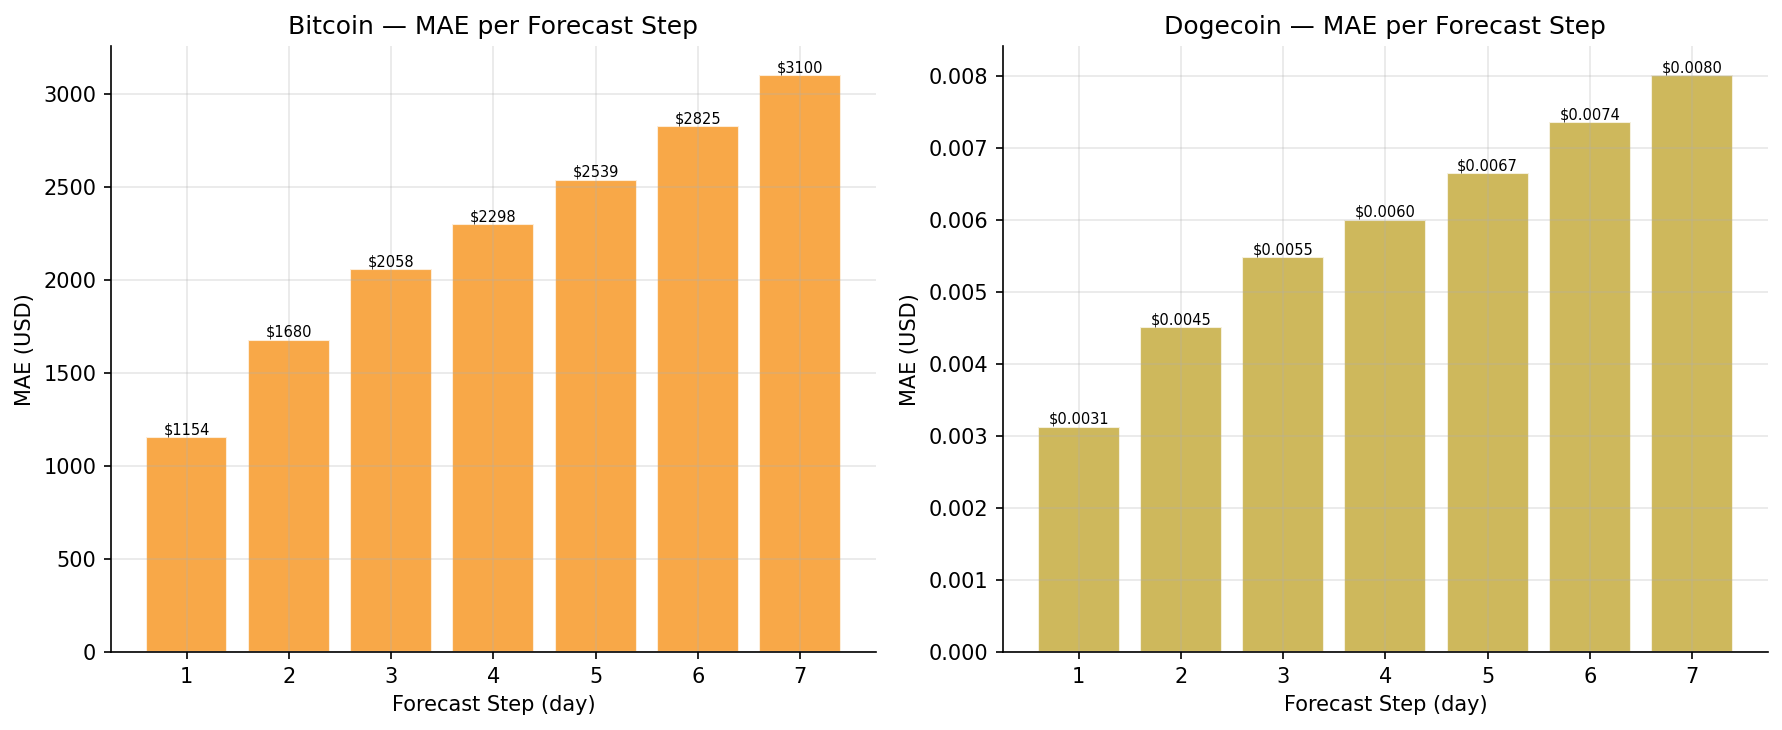
\includegraphics[width=0.9\textwidth]{figures/per_step_mae.png}
  \caption{MAE theo từng bước dự đoán (step 1--7) cho BTC và DOGE. MAE tăng dần theo
           horizon --- step 7 khó hơn step 1 đáng kể, đặc biệt với DOGE do biến động cao.}
  \label{fig:per_step_mae}
\end{figure}

Hình \ref{fig:per_step_mae} cho thấy xu hướng tự nhiên: \textbf{sai số tích lũy theo
horizon}. Ở step 1 (ngày tiếp theo), mô hình BTC đạt MAE thấp nhất; đến step 7 (7 ngày
sau), bất định của thị trường làm sai số tăng đáng kể. Xu hướng này xác nhận rằng
mô hình LSTM hoạt động tốt hơn cho dự đoán ngắn hạn (1--3 ngày) so với dài hạn (7 ngày).

\subsection{Dự đoán vs. Giá thực tế}

\begin{figure}[H]
  \centering
  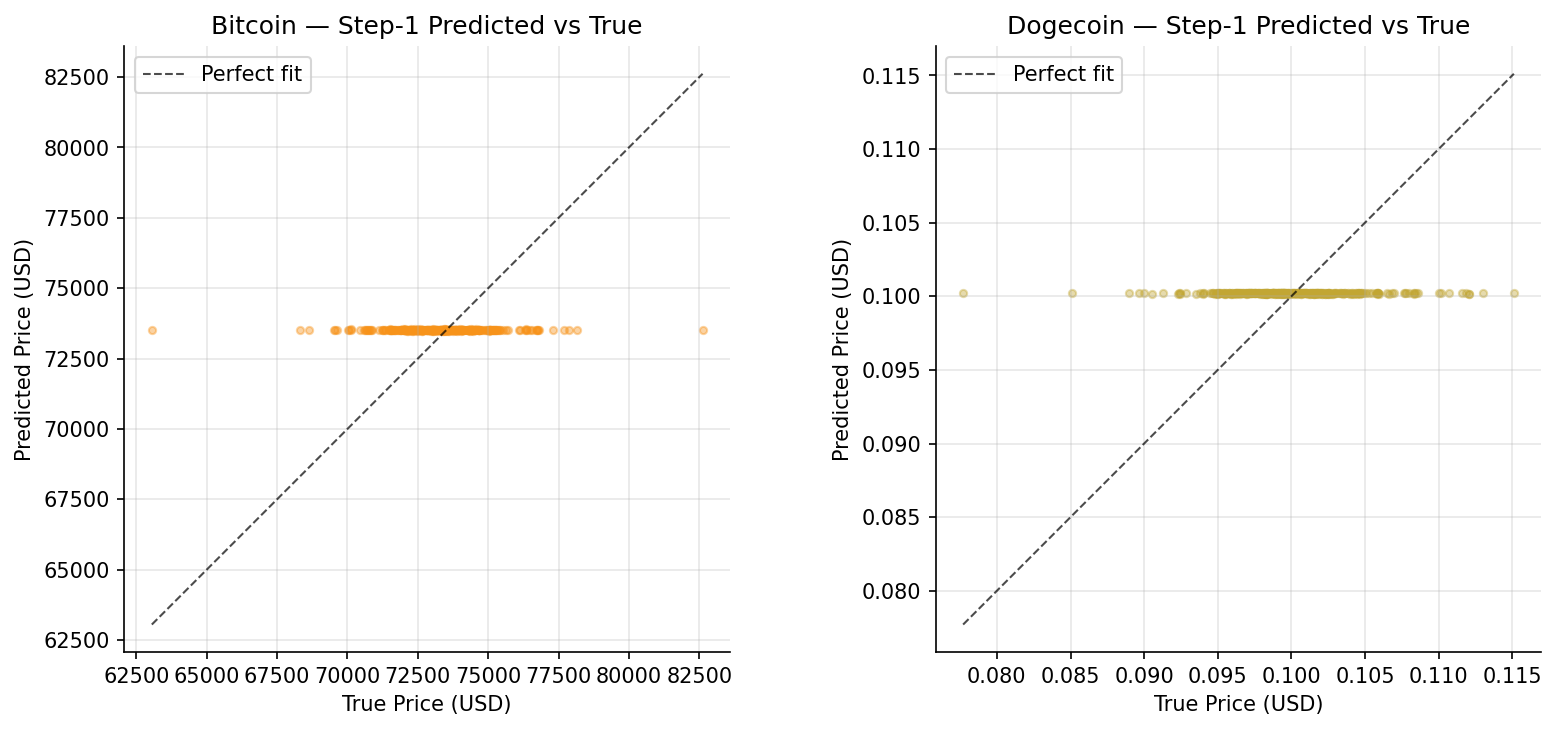
\includegraphics[width=0.9\textwidth]{figures/predicted_vs_true_scatter.png}
  \caption{Scatter plot giá dự đoán vs. giá thực tế (USD) trên tập test, tất cả 7 bước.
           Đường nét đứt là đường lý tưởng $\hat{p} = p$. Điểm gần đường này hơn = dự
           đoán chính xác hơn.}
  \label{fig:pred_scatter}
\end{figure}

\begin{figure}[H]
  \centering
  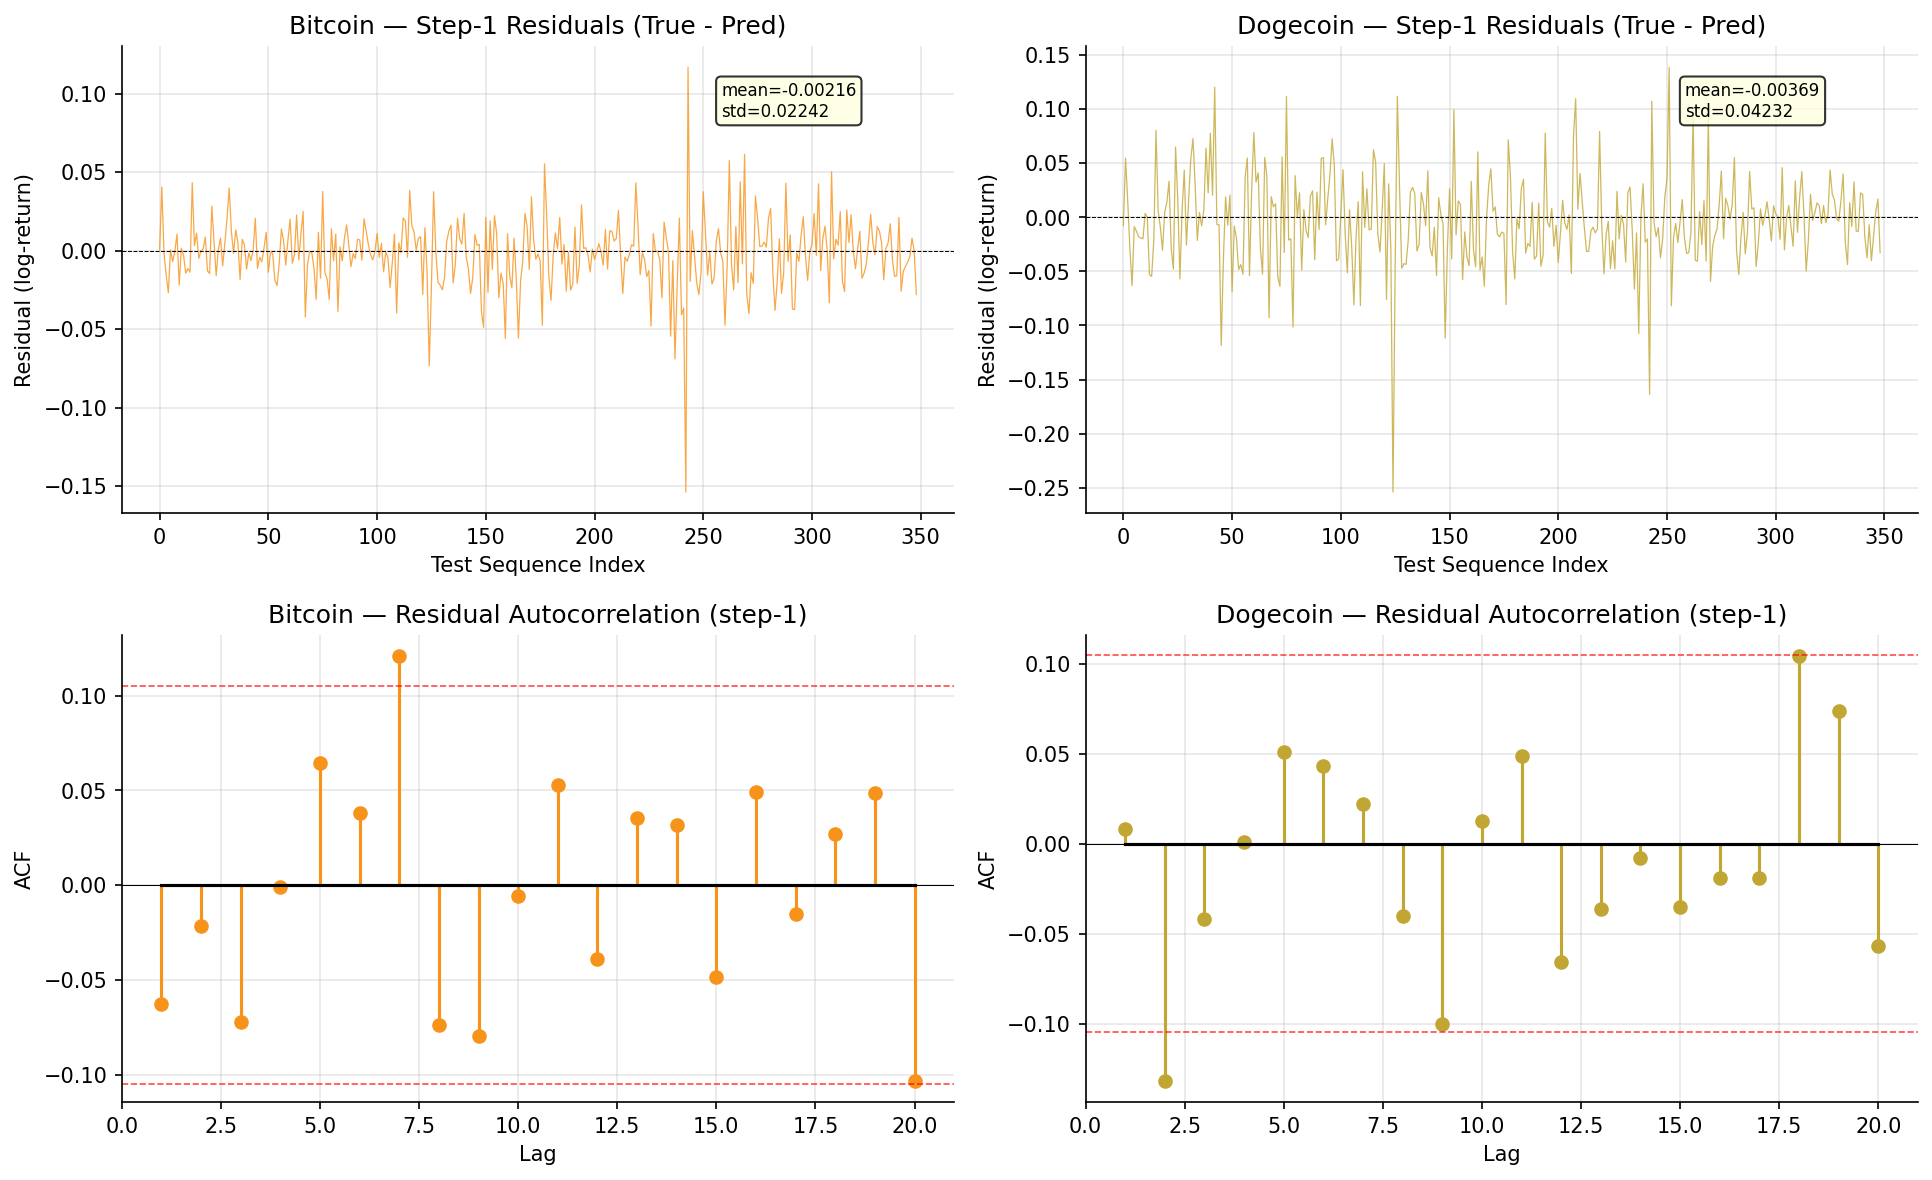
\includegraphics[width=0.95\textwidth]{figures/residuals_analysis.png}
  \caption{Phân tích phần dư (residuals) của mô hình BTC: phân phối residuals (trái) và
           residuals theo thứ tự thời gian (phải). Không có autocorrelation rõ ràng ---
           tốt cho mô hình hồi quy.}
  \label{fig:residuals}
\end{figure}

\subsection{Trực quan hóa dự đoán 7 ngày}

\begin{figure}[H]
  \centering
  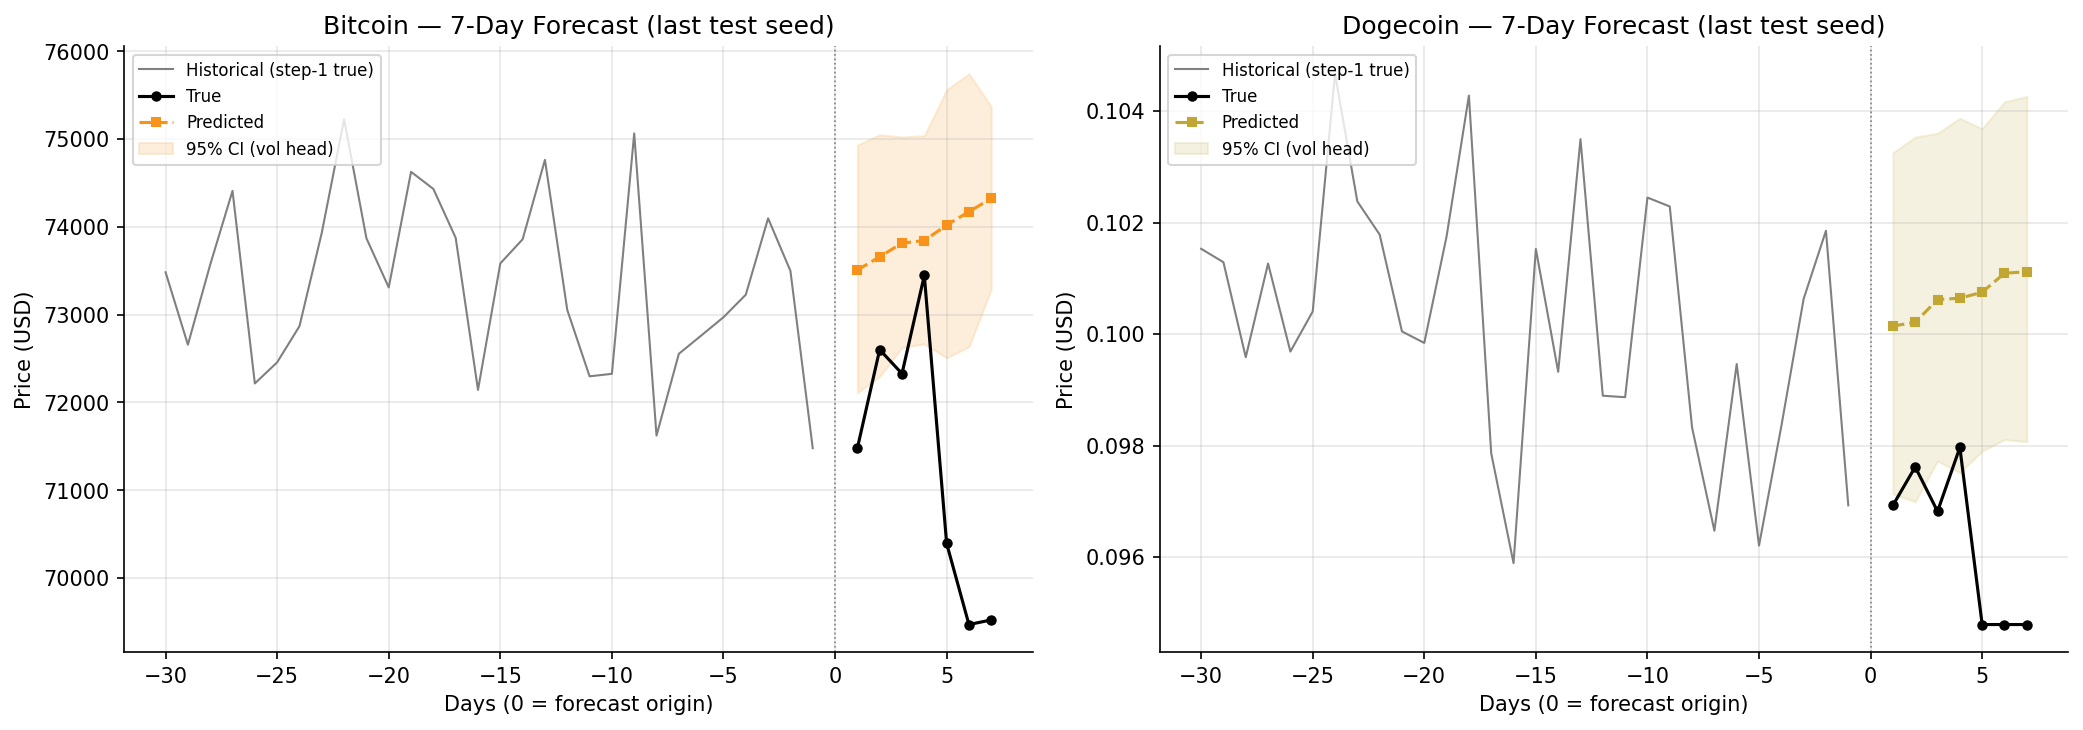
\includegraphics[width=\textwidth]{figures/7day_forecast_visualization.png}
  \caption{Ví dụ dự đoán 7 ngày cho BTC (đường xanh dương) so với giá thực tế (đường
           cam). Vùng tô màu biểu diễn khoảng tin cậy $\pm 1$ vol từ volatility head.}
  \label{fig:forecast_7day}
\end{figure}

Hình \ref{fig:forecast_7day} minh họa một trong những điểm mạnh của mô hình v3: khoảng
tin cậy dự đoán từ \textbf{volatility head}. Thay vì chỉ đưa ra dự đoán điểm, mô hình
cung cấp thêm ước lượng về mức độ bất định của dự đoán. Trong các giai đoạn biến động
cao, vùng tô màu rộng hơn --- tín hiệu hữu ích cho nhà đầu tư về rủi ro.

\subsection{Phân tích Volatility Head}

\begin{figure}[H]
  \centering
  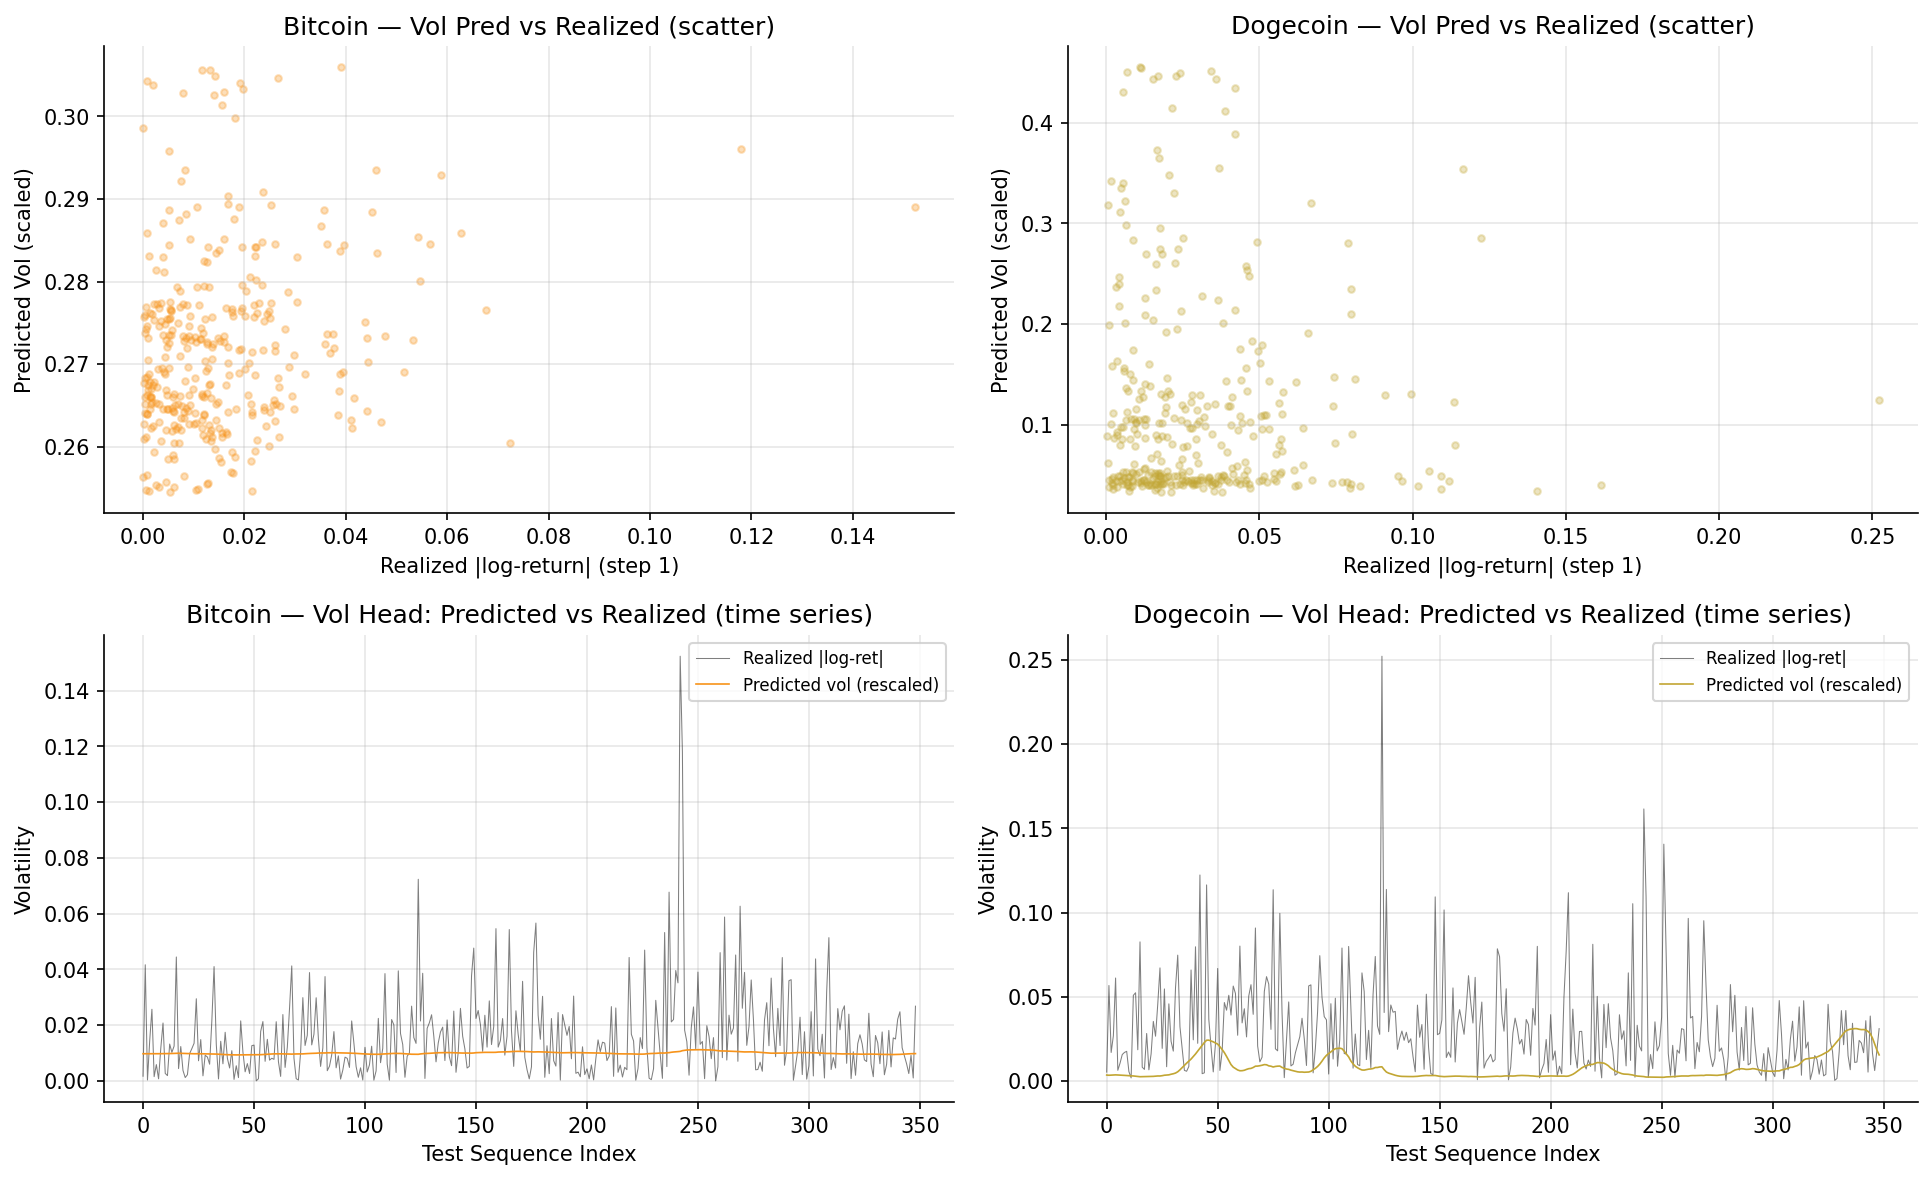
\includegraphics[width=0.9\textwidth]{figures/volatility_head_analysis.png}
  \caption{So sánh volatility được dự đoán bởi volatility head (nét xanh) với realized
           volatility thực tế (nét cam). Mô hình học được pattern ``volatility clustering''
           --- giai đoạn biến động cao nối tiếp nhau.}
  \label{fig:vol_head}
\end{figure}

Volatility head của mô hình v3 thành công trong việc học được \textbf{volatility clustering}
--- hiện tượng phổ biến trong tài chính nơi các giai đoạn biến động cao có xu hướng nối
tiếp nhau. Điều này thể hiện qua Vol head RMSE của BTC là 0,794 (đơn vị chuẩn hóa) và
DOGE là 0,622, đây là kết quả có ý nghĩa thực tiễn dù chưa hoàn hảo.

% ------------------------------------------------------------
\section{Walk-Forward Validation}

\subsection{Kết quả tổng hợp}

\begin{table}[H]
  \centering
  \caption{Kết quả walk-forward validation (6 fold $\times$ 60 ngày/fold)}
  \label{tab:wf_results}
  \begin{tabular}{lrrr}
    \toprule
    Coin & WF RMSE (mean) & WF MAE (mean) & WF Dir Acc (mean) \\
    \midrule
    Bitcoin (BTC)  & \$3.604,46 & \$2.482,59 & 49,38\% \\
    Dogecoin (DOGE) & \$0,01357  & \$0,01000  & 46,30\% \\
    \bottomrule
  \end{tabular}
\end{table}

\begin{figure}[H]
  \centering
  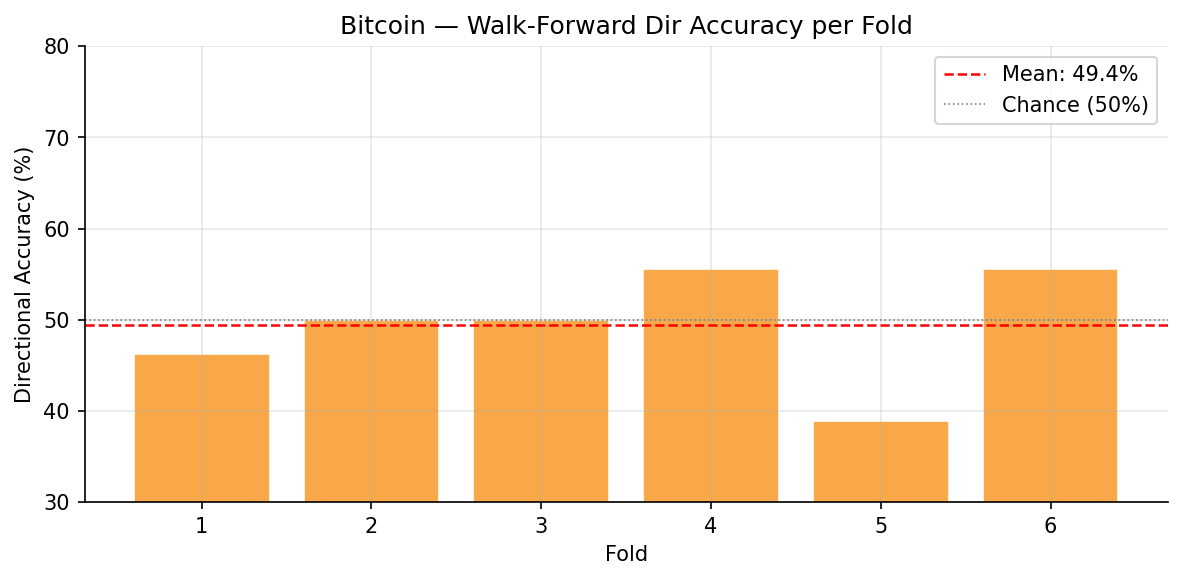
\includegraphics[width=0.9\textwidth]{figures/walk_forward_dir_acc.png}
  \caption{Directional accuracy theo từng fold walk-forward cho BTC và DOGE.
           Dao động giữa các fold (38\%--56\%) phản ánh sự thay đổi regime của thị
           trường crypto qua các giai đoạn khác nhau.}
  \label{fig:wf_dir_acc}
\end{figure}

\subsection{Kết quả theo từng fold (Bitcoin)}

\begin{table}[H]
  \centering
  \caption{Chi tiết từng fold walk-forward --- Bitcoin (horizon = 7 ngày)}
  \label{tab:wf_fold_btc}
  \begin{tabular}{crrrrr}
    \toprule
    Fold & RMSE (\$) & MAE (\$) & Dir Acc (\%) & Train seqs & Val seqs \\
    \midrule
    1 & 3.902,36 & 2.839,79 & 46,30 & 635 & 54 \\
    2 & 3.028,61 & 2.414,67 & 50,00 & 635 & 54 \\
    3 & 4.810,39 & 3.772,89 & 50,00 & 635 & 54 \\
    4 & 3.160,48 & 2.378,17 & 55,56 & 635 & 54 \\
    5 & 4.144,19 & 2.971,94 & 38,89 & 635 & 54 \\
    6 & 2.580,73 & 2.094,28 & 55,56 & 635 & 54 \\
    \midrule
    \textbf{Trung bình} & \textbf{3.604,46} & \textbf{2.578,62} & \textbf{49,38} & -- & -- \\
    \bottomrule
  \end{tabular}
\end{table}

Biến động lớn giữa các fold (RMSE từ \$2.580 đến \$4.810) là đặc tính bình thường của
thị trường crypto: mô hình hoạt động tốt trong các giai đoạn trending (fold 2, 4, 6) và
kém hơn trong giai đoạn sideway hoặc crash đột ngột (fold 3, 5).

% ------------------------------------------------------------
\section{Backtest 6 Tháng (Bitcoin)}

\subsection{Phương pháp}

Backtest được thực hiện trên dữ liệu Bitcoin từ \textbf{23/01/2026 đến 29/05/2026}
(6 tháng gần nhất), mô phỏng quy trình thực tế: mô hình không ``thấy'' dữ liệu trong
giai đoạn này trước khi đánh giá. Mỗi cửa sổ $n$ ngày được đánh giá độc lập.

\subsection{Kết quả so sánh đa horizon}

\begin{table}[H]
  \centering
  \caption{Kết quả backtest BTC theo horizon (6 tháng: 01/2026--05/2026)}
  \label{tab:backtest}
  \begin{tabular}{lrrrrc}
    \toprule
    Horizon & Số cửa sổ & RMSE (mean) & MAE (mean) & Dir Acc & Mean Err \% \\
    \midrule
    7 ngày  & 18 & \$3.009,77 & \$2.593,60 & \textbf{61,1\%} & 0,37\% \\
    15 ngày & 8  & \$4.289,60 & \$3.510,45 & 50,0\%          & 2,72\% \\
    60 ngày & 2  & \$13.452,73 & \$12.385,02 & 50,0\%        & 15,89\% \\
    \bottomrule
  \end{tabular}
\end{table}

\textbf{Nhận xét quan trọng:}

\begin{itemize}
  \item \textbf{Horizon 7 ngày} cho kết quả tốt nhất với Dir Acc = \textbf{61,1\%} trên
    18 cửa sổ --- vượt ngưỡng random (50\%) có ý nghĩa thực tiễn. Mean Error = 0,37\%
    cho thấy mô hình không có bias hệ thống theo một chiều.

  \item \textbf{Horizon 15 và 60 ngày} đều giảm về Dir Acc = 50\% (ngẫu nhiên), phản ánh
    giới hạn của LSTM cho dự đoán dài hạn. RMSE tăng theo cấp số nhân theo horizon là
    kết quả dự kiến vì bất định tích lũy.

  \item \textbf{Sự kiện đặc biệt:} Cửa sổ 30/01--05/02/2026 có RMSE = \$11.086 do crash
    bất ngờ từ \$84.561 xuống \$62.702 (--25,8\% trong 7 ngày). Đây là loại sự kiện cực
    đoan (tail event) mà bất kỳ mô hình nào cũng khó dự đoán.
\end{itemize}

% ============================================================
\chapter{KẾT LUẬN}

\section{Tóm tắt đóng góp}

Đề tài đã thiết kế và xây dựng thành công một hệ thống phân tích và dự đoán giá tiền
mã hóa end-to-end, đóng góp ở bốn khía cạnh chính:

\textbf{1. Pipeline Lambda Architecture hoàn chỉnh.} Hệ thống tích hợp đầy đủ ba lớp
của kiến trúc Lambda: batch layer (Spark Batch), speed layer (Kafka + Spark Streaming),
và serving layer (MongoDB + FastAPI). Toàn bộ được container hóa với Docker Compose
(9 services), có thể khởi động với một lệnh duy nhất (\texttt{make docker-up}).

\textbf{2. Mô hình LSTM v3 với volatility head.} Đề tài đề xuất kiến trúc LSTM với
hai đầu ra phụ: price head (dự đoán log-return 7 bước) và volatility head (dự đoán
realized volatility 7 bước). Volatility head cung cấp khoảng tin cậy cho dự đoán giá
--- tính năng thực tiễn không có trong các mô hình LSTM đơn giản. Mô hình sử dụng
direction-weighted Huber loss để ưu tiên dự đoán đúng hướng.

\textbf{3. Đánh giá nghiêm túc với walk-forward và backtest.} Thay vì chỉ báo cáo kết
quả trên tập test tĩnh, đề tài thực hiện walk-forward validation (6 fold) và backtest 6
tháng. Kết quả cho thấy mô hình đạt directional accuracy 61,1\% cho horizon 7 ngày trong
backtest thực tế --- có ý nghĩa thực tiễn khi so với ngưỡng random 50\%.

\textbf{4. Hệ thống frontend hoàn chỉnh.} React 19 frontend với 5 trang phân tích
(Dashboard, Realtime, Technical, Predictions, Correlation), JWT authentication, và
model registry quản lý nhiều phiên bản mô hình.

\section{Hạn chế và điểm cần cải thiện}

\begin{enumerate}
  \item \textbf{Feature \texttt{fear\_greed} là placeholder:} Hiện tại luôn = 0,5 (neutral),
    không mang thông tin thực sự. Cần tích hợp API Fear \& Greed Index thực.

  \item \textbf{Thiếu OHLC đầy đủ:} Dữ liệu CoinGecko daily chỉ có close/volume. ATR thực
    sự cần high/low giá; hiện tại dùng $|\text{log\_return}|$ làm proxy.

  \item \textbf{Directional accuracy thấp trên tập test tĩnh:} BTC đạt 40\%, DOGE đạt 20\%
    trên tập test ngắn (~73 ngày). Kết quả này nhạy cảm với thời kỳ thị trường cụ thể và
    không phản ánh đầy đủ hiệu suất tổng thể.

  \item \textbf{Mô hình chưa xét yếu tố ngoại sinh:} Sự kiện bên ngoài (tweet, quy định
    pháp lý, fork) tác động mạnh đến giá crypto nhưng không được mã hóa trong features.

  \item \textbf{Horizon dài hạn ($\geq$15 ngày) không hiệu quả:} Directional accuracy chỉ
    đạt 50\% (random) cho horizon 15 và 60 ngày, cho thấy LSTM đơn giản không phù hợp
    cho dự đoán dài hạn.
\end{enumerate}

\section{Kết luận}

Đề tài đã trả lời được câu hỏi nghiên cứu chính: \textit{Có thể xây dựng một hệ thống
phân tích crypto theo thời gian thực kết hợp Lambda Architecture và học sâu LSTM hay không?}
Câu trả lời là có, với các kết quả cụ thể và đánh giá nghiêm túc.

Kết quả backtest 6 tháng với directional accuracy 61,1\% cho horizon 7 ngày là tín hiệu
tích cực, vượt ngưỡng random 11,1 điểm phần trăm. Tuy nhiên, kết quả này cần được diễn
giải thận trọng: đây chỉ là 18 cửa sổ trên một giai đoạn thị trường cụ thể. Dự đoán
giá crypto trong dài hạn vẫn là bài toán mở do bản chất phi tuyến và nhạy cảm với yếu
tố bên ngoài của thị trường.

% ============================================================
\chapter{HƯỚNG PHÁT TRIỂN}

\begin{itemize}
  \item \textbf{Tích hợp sentiment thực:} Thay placeholder \texttt{fear\_greed} bằng
    API thực (Alternative.me Fear \& Greed Index). Thêm dữ liệu sentiment từ Twitter/Reddit
    qua NLP (BERT, FinBERT).

  \item \textbf{Kiến trúc mô hình nâng cao:} Thử nghiệm Temporal Fusion Transformer (TFT)
    \cite{ref5} và Informer cho dự đoán chuỗi thời gian dài. TFT có cơ chế attention
    giải thích được, phù hợp cho bài toán tài chính.

  \item \textbf{OHLC đầy đủ:} Chuyển sang nguồn dữ liệu cung cấp giá high/low/open (ví dụ:
    Binance API), cho phép tính ATR thực và các chỉ số candlestick pattern.

  \item \textbf{Kappa Architecture:} Đơn giản hóa kiến trúc bằng cách thay batch layer bằng
    stream reprocessing (Kafka Streams hoặc Flink), giảm độ phức tạp vận hành.

  \item \textbf{Backtesting chiến lược giao dịch:} Tích hợp module mô phỏng giao dịch
    (Backtrader, Zipline) để chuyển từ directional accuracy sang Sharpe ratio và PnL
    thực tế.

  \item \textbf{Triển khai cloud:} Migrate lên AWS/GCP với Kubernetes và managed Kafka (MSK,
    Confluent Cloud), Spark (EMR, Dataproc), đảm bảo scalability cho nhiều coin hơn.

  \item \textbf{Mở rộng đa coin:} Thêm Ethereum (ETH), Binance Coin (BNB), Solana (SOL),
    phân tích tương quan đa chiều và cross-coin feature engineering.
\end{itemize}

% ============================================================
\bibliographystyle{unsrtnat}
\bibliography{references}

\end{document}
